\documentclass[a4paper,12pt]{article}

% ============================= PAKIETY ================================
   \usepackage[T1]{fontenc}
   \usepackage{polski}
   \usepackage[utf8]{inputenc}
   \usepackage{lmodern}
   \usepackage{graphicx}
   \usepackage{here}
   \usepackage{geometry}
   \usepackage{setspace}
   \usepackage{amsmath}
   \usepackage{amsthm}
   \usepackage{eucal}
   \usepackage{amssymb}
   \usepackage{mathrsfs}
   \usepackage{setspace}
   \usepackage{multirow}
   \usepackage{tabularx}
   \usepackage{hhline}
   \usepackage{subcaption}
   \usepackage{wrapfig}
   \usepackage{minted}
   \usepackage{siunitx}
   \usepackage{enumerate}
   \usepackage[justification=centering,font=small]{caption}
% ======================================================================


\linespread{1} %1.3 do interlinii 1.5

\begin{document}

% ========================== STRONA TYTUŁOWA============================
   \thispagestyle{empty}
   \newgeometry{tmargin=2.5cm,bmargin=2.5cm,lmargin=2.5cm,rmargin=2.5cm}
   
   \begin{flushright}
      \rm \large{Warszawa 2014}
   \end{flushright}
  \vskip0.5cm
   
   \begin{flushleft}
        \begin{tabular}{c}
         \large{Politechnika Warszawska}\\
         \large{Wydział Elektroniki i Technik Informacyjnych}\\
         \large{Instytut Automatyki i Informatyki Stosowanej}
      \end{tabular}
   \end{flushleft}
   \vskip1cm
   
   \begin{figure}[ht]
      \centering
      
\includegraphics{img/logo_PW.jpg}
   \end{figure}
   \vskip1cm
   
   \begin{center}
      \large{Łukasz Jendrzejek}\\
      \large{Paweł Świokło}\\
   \end{center}
   \vskip0.5in

   \begin{center}
      \large{SZTUCZNA INTELIGENCJA W AUTOMATYCE - PROJEKT}
   \end{center}
   \vskip1cm

   \begin{center}
   \large{\textbf{Sterowanie kaskadą zbiorników z wykorzystaniem modelu rozmytego obiektu.}}
   \end{center}

   \newpage
   \thispagestyle{empty}
% ======================================================================
\tableofcontents


\newpage
\section{Opis obiektu}

\paragraph{}
Obiektem rozważanym w niniejszym zadaniu jest kaskada dwóch zbiorników. Zadanie sterowania polega na odpowiednim ustalaniu dopływającego strumienia medium tak, aby stabilizować poziom tego medium w drugim zbiorniku.
Schemat obiektu został ukazany na rysunku \ref{img:schemat}.
Są na nim ukazane dwa strumienie dostarczające medium:

\begin{itemize}
   \item strumień sterowany $F_{1in}$,
   \item strumień zakłócający $F_D$.
\end{itemize}

\begin{figure}[h]
   \centering
   \begin{subfigure}[h]{0.65\textwidth}
      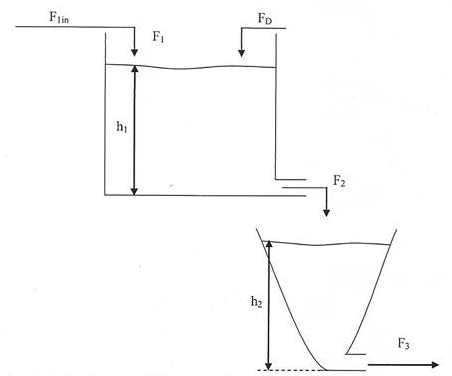
\includegraphics[width=\textwidth]{img/schemat.jpg}
   \end{subfigure}
   \caption{Graficzny schemat struktury rozważanej kaskady zbiorników.}
   \label{img:schemat}
\end{figure}

\noindent Poziom wypełnienia zbiorników reprezentowany jest przez parametry odpowiednio $h_1$ i $h_2$.
Ważnym elementem występującym niejawnie na schemacie jest opóźnienie strumienia wejściowego.
Wartością sterowaną jest dopływ reprezentowany przez $F_{1in}$, a strumień dopływający do pierwszego strumienia w danej chwili określany jest przez wielkość $F_1$.
\newline
\newline
Wraz z obiektem zostały dostarczone równania opisujące występujące zależności:

\begin{equation}
   \left\lbrace
   \begin{array}{l}
      \begin{matrix}\frac{\text{d}V_1}{\text{d}t}\end{matrix} ~=~ F_1 ~+~ F_D ~-~ F_2(h_1)\\[0.2cm]
      \begin{matrix}\frac{\text{d}V_2}{\text{d}t}\end{matrix} ~=~ F_2(h_1) ~-~ F_3(h_2)\\[0.2cm]
      F_2(h_1) ~=~ \alpha_1 \cdot \sqrt{h_1} \\[0.2cm]
      F_3(h_2) ~=~ \alpha_2 \cdot \sqrt{h_2} \\[0.2cm]
      V_1(h_1) ~=~ A_1 \cdot h_1 \\[0.2cm]
      V_2(h_2) ~=~ C_2 \cdot h_2^2 \\[0.2cm]
      F_1(t) ~=~ F_{1in}(t-\tau) \\[0.2cm]
   \end{array}
   \right.
\end{equation}

\noindent Stałe opisujące zbiornik wynoszą odpowiednio:

\begin{itemize}
   \item $A_1 ~=~ 550~\text{cm}^2$
   \item $C_2 ~=~ 0.8$
   \item $\alpha_1 ~=~ 28$
   \item $\alpha_2 ~=~ 16$
\end{itemize}

\noindent a punkt pracy, wokół którego odbywać się będzie linearyzacja i sterowanie obiektu dany jest parametrami o wartościach:

\begin{itemize}
   \item $F_1 ~=~ 100~\frac{\text{cm}^3}{s}$
   \item $F_D ~=~ 20~\frac{\text{cm}^3}{s}$
   \item $\tau ~=~ 60~\text{s}$
   \item $h_2 ~=~ 56.25~\text{cm}$
\end{itemize}

\section{Modelowanie otrzymanego obiektu}
\paragraph{}
Pierwszą częścią projektu było skupienie się na samym obiekcie i sposobach jego modelowania.
W pierwszej kolejności obiekt zostanie wiernie odwzorowany, wykorzystane będą bezpośrednio podane równania różniczkowe dostarczone wraz z treścią projektu.
Po analizie zachowania obiektu i sprawdzeniu jego odpowiedzi na skoki wartości sygnałów na wejściach dokonana zostanie linearyzacja w punkcie pracy, a następnie dyskretyzacja uzyskanego modelu liniowego w celu wykorzystania go do regulacji.
Ostatnim etapem modelowania będzie utworzenie modelu rozmytego obiektu.


\subsection{Symulacja pełnego, nieliniowego obiektu}

\begin{figure}[h]
   \centering
   \begin{subfigure}[h]{0.45\textwidth}
      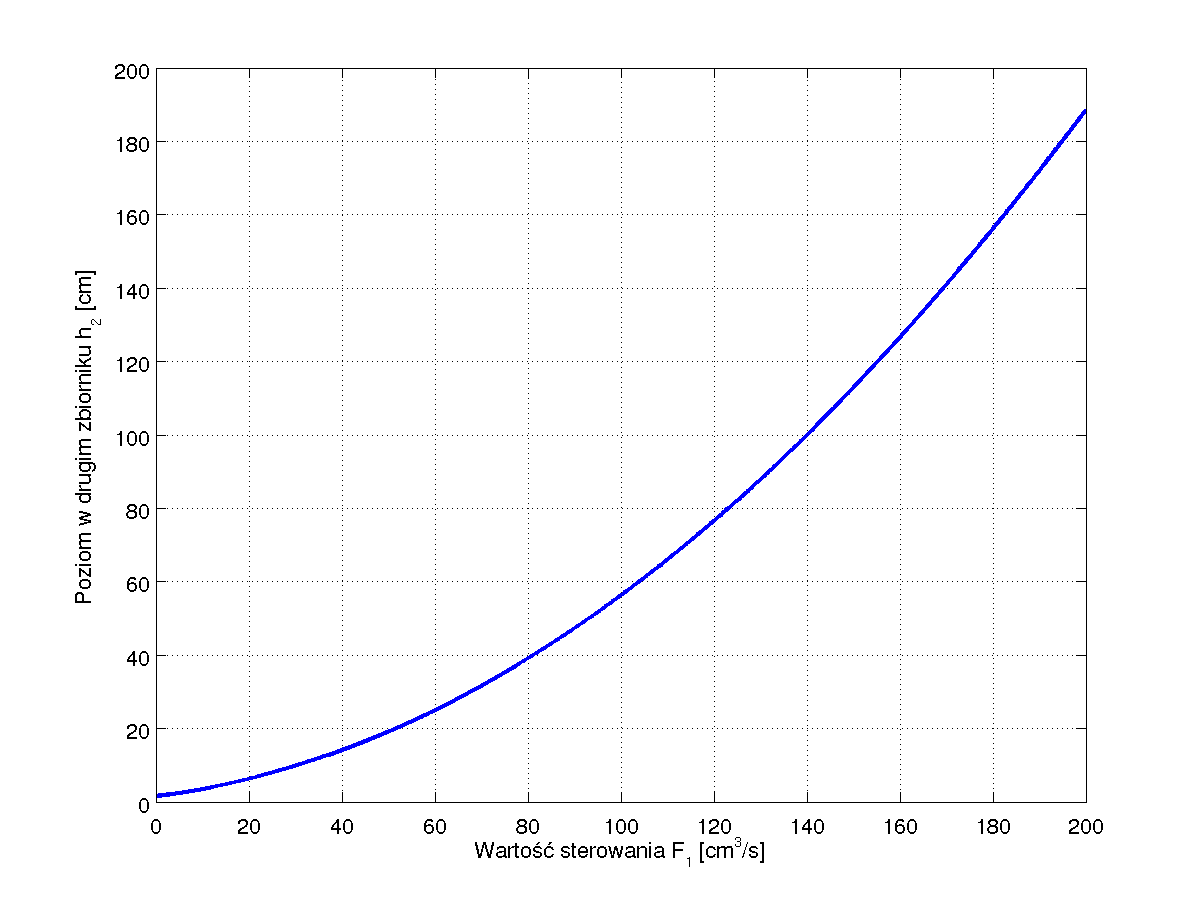
\includegraphics[width=\textwidth]{img/char_stat_1.png}
      \caption{Charakterystyka statyczna toru wejście-wyjście}
   \end{subfigure}
   \begin{subfigure}[h]{0.45\textwidth}
      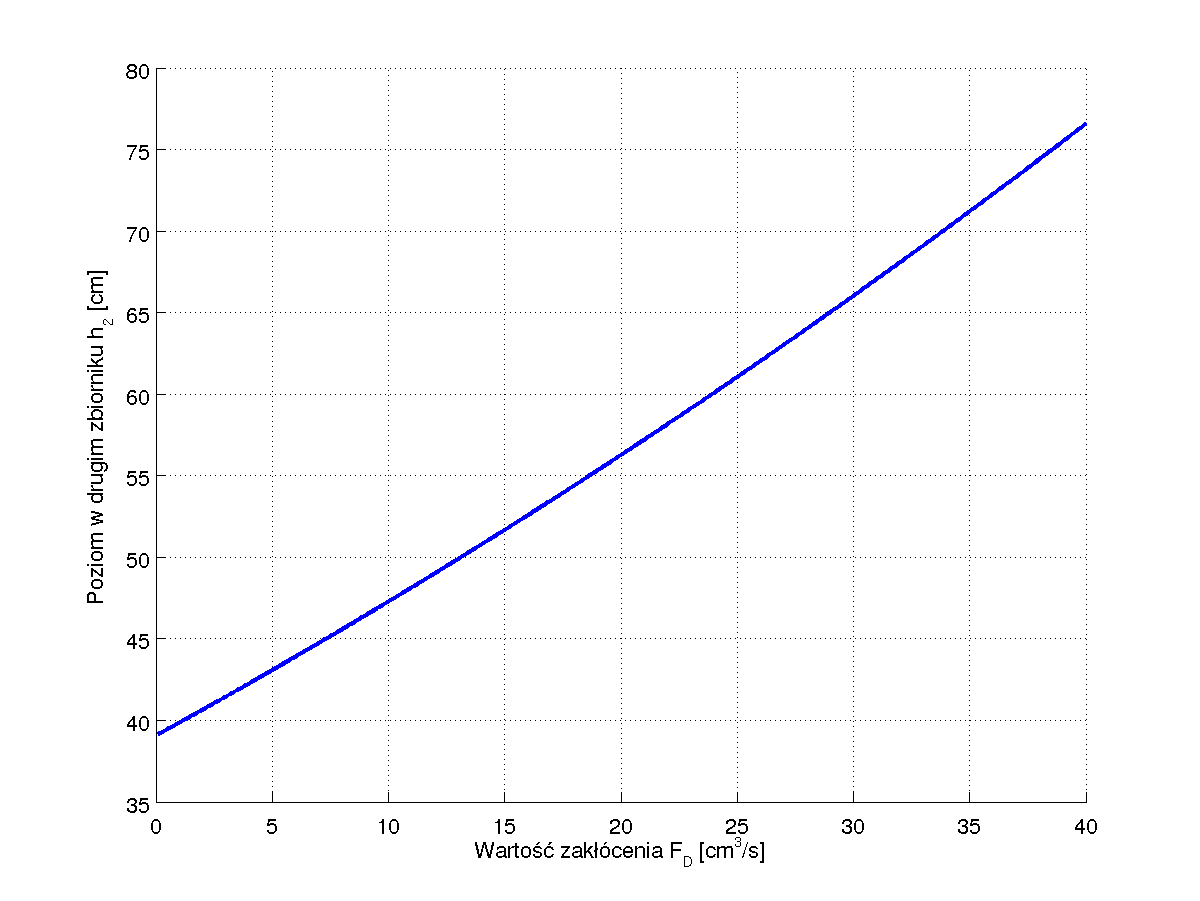
\includegraphics[width=\textwidth]{img/char_stat_2.png}
      \caption{Charakterystyka statyczna toru zakłócenie-wyjście.}
   \end{subfigure}
   \caption{Charakterystyki statyczne obiektu.}
   \label{img:char_stat}
\end{figure}

\paragraph{}
Opis matematyczny obiektu wyrażony w postaci równań różniczkowych został rozwiązany za pomocą funkcji \texttt{ode45} programu Matlab posługującej się metodą Rungego-Kutty.
Pierwszym krokiem było wykreślenie charakterystyki statycznej obiektu.
W tym celu obiekt był wielokrotnie symulowany aż do ustalenia się odpowiedzi na jego wyjściu na stałe sterowanie.
Wyniki symulacji zostały przedstawione na rysunku \ref{img:char_stat}.

\paragraph{}
Przebieg charakterystyki statycznej obrazuje zmianę wzmocnienia statycznego obiektu.
Można zauważyć silną nieliniowowść w torze wejście-wyjście, tak więc adekwatność modelu liniowego będzie silnie ograniczona do pewnego sąsiedztwa punktu pracy.

\paragraph{}
Następnie sprawdzona została nieliniowość dynamiczna obiektu.
Rysunki \ref{img:symulacja_obiektu_1} i \ref{img:symulacja_obiektu_2} przedstawiają odpowiedzi obiektu na skoki wartości odpowiednio sterowania i zakłócenia.
Wynika z nich, że obiekt wyraźnie szybciej reaguje na zmniejszanie dopływu do zbiorników.

\begin{figure}[h]
   \centering
   \begin{subfigure}[h]{0.45\textwidth}
      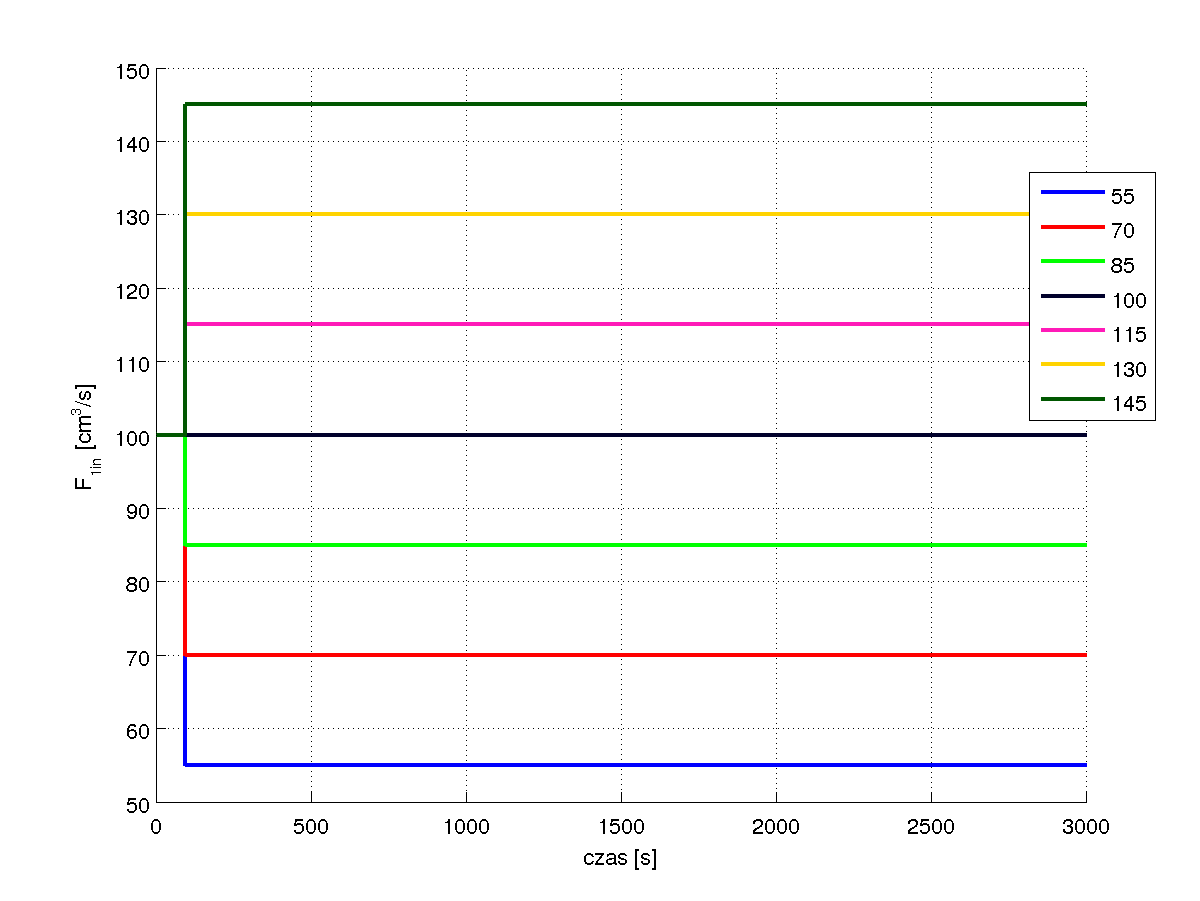
\includegraphics[width=\textwidth]{img/symulacja_obiektu_1a.png}
      \caption{Zmiany natężenia dopływającego strumienia sterującego.}
   \end{subfigure}
   \begin{subfigure}[h]{0.45\textwidth}
      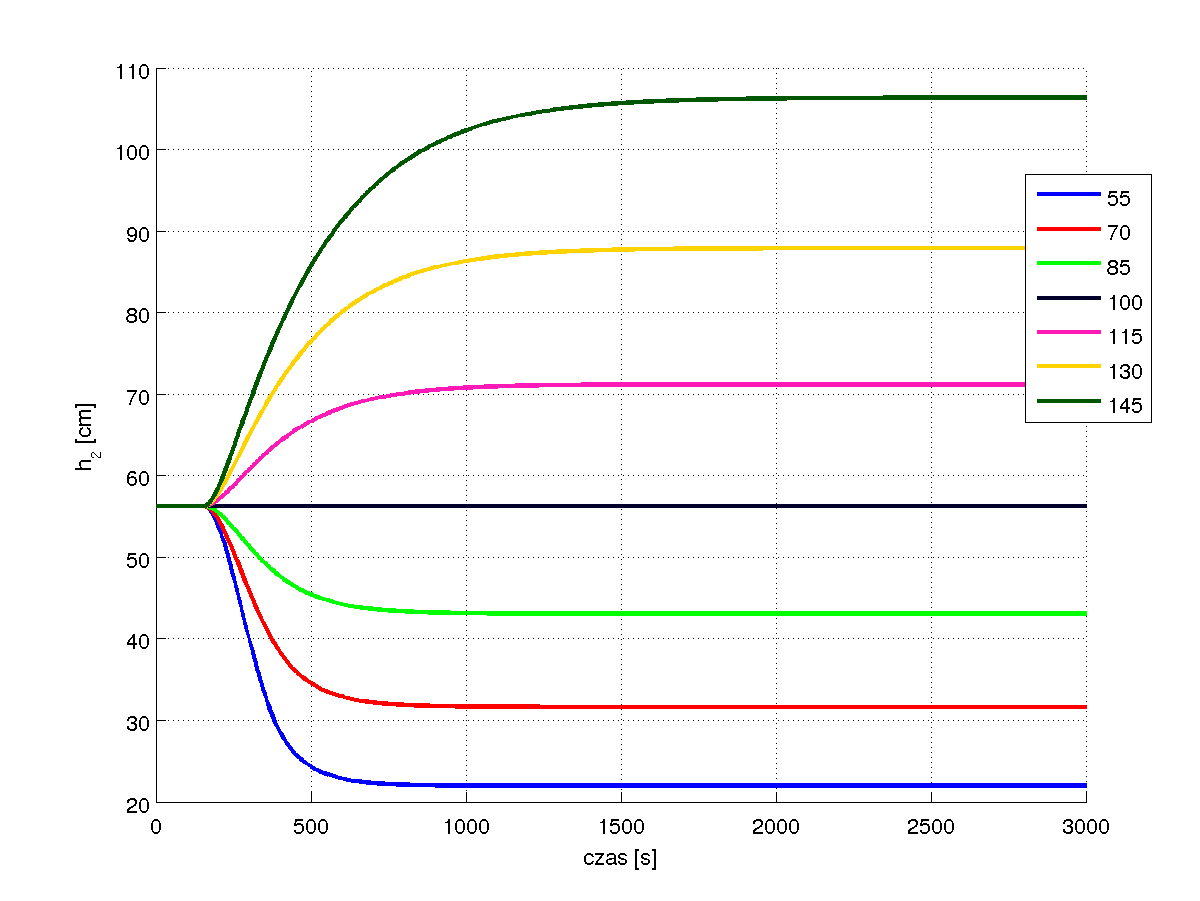
\includegraphics[width=\textwidth]{img/symulacja_obiektu_1b.png}
      \caption{Odpowiedzi obiektu na skok wartości na wejściu.}
   \end{subfigure}
   \caption{Reakcja obiektu na zmianę wielkości dopływającego strumienia sterującego.}
   \label{img:symulacja_obiektu_1}
\end{figure}

\begin{figure}[h]
   \centering
   \begin{subfigure}[h]{0.45\textwidth}
      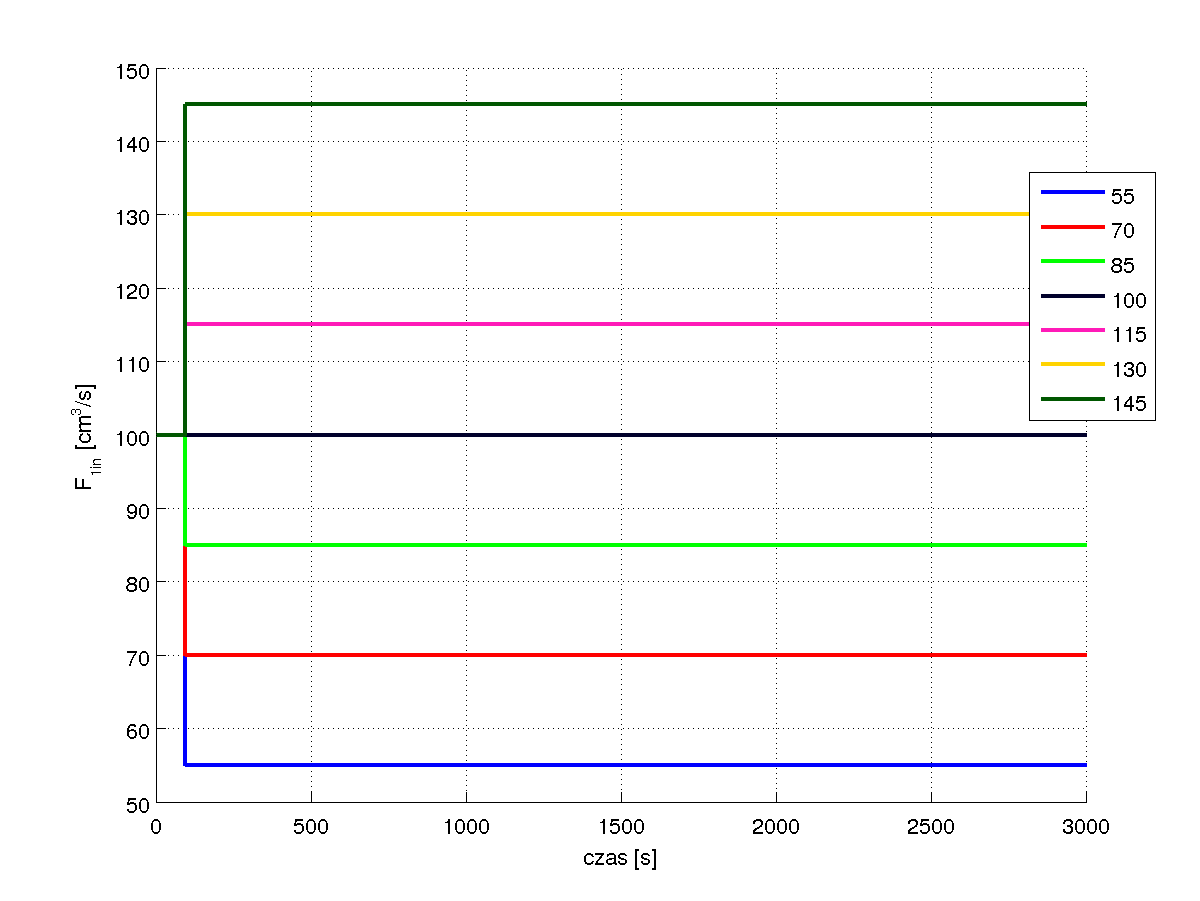
\includegraphics[width=\textwidth]{img/symulacja_obiektu_1a.png}
      \caption{Zmiany natężenia dopływającego strumienia zakłócającego}
   \end{subfigure}
   \begin{subfigure}[h]{0.45\textwidth}
      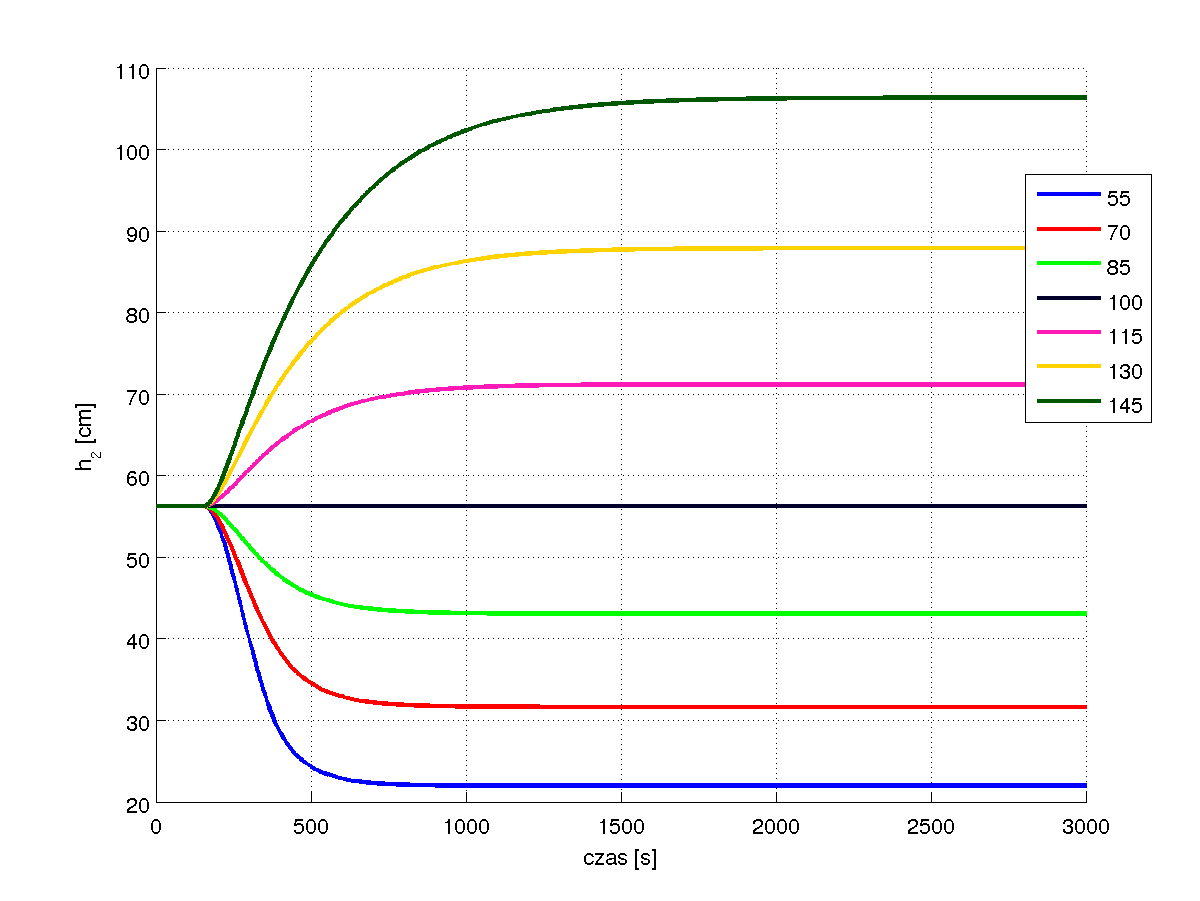
\includegraphics[width=\textwidth]{img/symulacja_obiektu_1b.png}
      \caption{Odpowiedzi obiektu na skok wartości zakłócenia}
   \end{subfigure}
   \caption{Reakcja obiektu na zmianę wielkości dopływającego strumienia zakłócającego.}
   \label{img:symulacja_obiektu_2}
\end{figure}

\paragraph{}
Powyższe wykresy ilustrują poprawne działanie modelu opisanego równaniami różniczkowymi.
Pełne modele nieliniowe opisujące rzeczywistość równaniami różniczkowymi ciężko jednak na ogół wykorzystać w algorytmie sterowania, dlatego zostaną sporządzone modele liniowe i rozmyte, które zostaną bezpośrednio wykorzystane do syntezy regulatorów obiektu.

\subsection{Liniowy model ciągły}
\paragraph{}
Zabieg linearyzacji polega na utworzeniu modelu liniowego rozważanego obiektu sterowania wokół określonego punktu pracy.
Z racji tego, że model liniowy charakteryzuje się stałym wzmocnieniem, stanowi on dobre przybliżenie modelu nieliniowego jedynie w pewnym otoczeniu punktu pracy.
Zabieg ten powoduje, że tracimy na dokładności modelu, którym się posługujemy, jednak zyskujemy na znacznym uproszczeniu reguł sterowania, ponieważ teoria sterowania stacjonarnych obiektów liniowych ma silne dowody stabilności.

\paragraph{}
Jedną z powszechnie stosowanych metod linearyzacji jest linearyzacja lokalna.
Jeżeli funkcja w przestrzeni $n$ wymiarowej $R^n$ jest różniczkowalna i ma w otoczeniu danego punktu $x_0$ ciągłe pochodne względem swoich argumentów, można dokonać lokalnego przybliżenia wartości $f(x)$ w punkcie $x$ bliskim $x_0$ w postaci zależności:

\begin{equation}
   f_{lin}(x) ~=~ f(x_0) ~+~ \left.\frac{\text{d}f(x)}{\text{d}x}\right|_{x=x_0} \cdot (x - x_0)
\end{equation}

\paragraph{}
Linearyzację należy rozpocząć od przekształcenia równań obiektu.
Równania powinny zostać doprowadzone do postaci, w której po lewej stronie występuje pochodna zmiennej, a po prawej stronie zmienna ta występuje jawnie.
Zatem dokonując odpowiednich przekształceń algebraicznych otrzymane zostały następujące nieliniowe równania stanu obiektu:

\begin{equation}
   \left\lbrace
   \begin{array}{rcl}
      \begin{matrix}\frac{\text{d}V_1}{\text{d}t}\end{matrix} & = & F_1 ~+~ F_D ~-~ \alpha_1\cdot\sqrt{\frac{V_1}{A_1}}\\[0.1cm]
      \begin{matrix}\frac{\text{d}V_2}{\text{d}t}\end{matrix} & = & \alpha_1\cdot\sqrt{\frac{V_1}{A_1}} ~-~ \alpha_2\cdot\sqrt[4]{\frac{V_2}{C_2}}\\[0.1cm]
   \end{array}
   \right.
\end{equation}

\noindent Pełny opis obiektu należy uzupełnić jeszcze o równanie wyjścia, które jest następujące:

\begin{equation}
   h_2 ~=~ \sqrt{ \begin{matrix} \frac{V_2}{C_2} \end{matrix} }
\end{equation}

\noindent Oznaczając powyższe funkcje w następujący sposób:

\begin{equation}
   \left\lbrace
   \begin{array}{rcl}
      f_1(F_1, V_1, V_2) & = & \begin{matrix}\frac{\text{d}V_1}{\text{d}t}\end{matrix} \\[0.1cm]
      f_2(F_1, V_1, V_2) & = & \begin{matrix}\frac{\text{d}V_2}{\text{d}t}\end{matrix} \\[0.1cm]
      g(F_1, V_1, V_2) & = & h_2 \\[0.1cm]
   \end{array}
   \right.
\end{equation}

\noindent zostały wyznaczone analitycznie pochodne cząstkowe funkcji:

\begin{equation}
   \begin{array}{rcl}
      \begin{matrix} \frac{\text{d}f_1}{\text{d}F_1} \end{matrix} & = & 1 \\[0.1cm]
      \begin{matrix} \frac{\text{d}f_1}{\text{d}V_1} \end{matrix} & = & -\begin{matrix} \frac{\alpha_1}{2} \end{matrix} \cdot \sqrt{ \begin{matrix} \frac{1}{A_1 \cdot V_1} \end{matrix} } \\[0.1cm]
      \begin{matrix} \frac{\text{d}f_1}{\text{d}V_2} \end{matrix} & = & 0 \\[0.1cm]
   \end{array}
\end{equation}

\addtocounter{equation}{-1}

\begin{equation}
   \begin{array}{rcl}
      \begin{matrix} \frac{\text{d}f_2}{\text{d}F_1} \end{matrix} & = & 0 \\[0.1cm]
      \begin{matrix} \frac{\text{d}f_2}{\text{d}V_1} \end{matrix} & = & \begin{matrix} \frac{\alpha_1}{2} \end{matrix} \cdot \sqrt{ \begin{matrix} \frac{1}{A_1 \cdot V_1} \end{matrix} } \\[0.1cm]
      \begin{matrix} \frac{\text{d}f_2}{\text{d}V_2} \end{matrix} & = & -\begin{matrix} \frac{\alpha_2}{4} \end{matrix} \cdot \sqrt[4]{ \begin{matrix} \frac{1}{C_2 \cdot V_2^3} \end{matrix} } \\[0.1cm]
      \begin{matrix} \frac{\text{d}g}{\text{d}V_1} \end{matrix} & = & 0 \\[0.1cm]
      \begin{matrix} \frac{\text{d}g}{\text{d}V_2} \end{matrix} & = & \begin{matrix} \frac{1}{2} \end{matrix} \cdot \sqrt{ \begin{matrix} \frac{1}{C_2 \cdot V_2} \end{matrix} } \\[0.1cm]
   \end{array}
\end{equation}

\paragraph{}
Model liniowy przyrostowy w postaci równania stanu - równanie wyjścia jest postaci:

\begin{equation}
   \begin{gathered}
      \dot{\boldsymbol{x}} ~=~ \boldsymbol{Ax} + \boldsymbol{Bu}\\[0.1cm]
      \boldsymbol{y} ~=~ \boldsymbol{Cx} + \boldsymbol{Du}
   \end{gathered}
\end{equation}

\noindent gdzie:

\begin{equation}
   \begin{gathered}
      \boldsymbol{x} ~=~ \left[ 
      \begin{array}{c}
         V_1 - V_{10}\\
         V_2 - V_{20}\\
      \end{array}
      \right],
      ~~~~~~~~~~~~~
      \boldsymbol{u} ~=~ \left[ 
      \begin{array}{c}
         F_1 - F_{10}
      \end{array}
      \right]
      \\
      \boldsymbol{y} ~=~ \left[ 
      \begin{array}{c}
         h_2 - h_{20}
      \end{array}
      \right]
   \end{gathered}
\end{equation}

\paragraph{}
Macierze $\boldsymbol{A}, \boldsymbol{B}$ i $\boldsymbol{C}$ składają się więc z następujących elementów (dla uproszczenia zapisu przyjęto oznaczenie $p.p.$ jako warunek zdefiniowany przez punkt pracy podany w treści polecenia):

\begin{equation}
   \begin{gathered}
      \boldsymbol{A} ~=~
      \left[
         \begin{array}{cc}
            \left. \frac{\partial f_1}{\partial V_1} \right|_{p.p.} & 
               \left. \frac{\partial f_1}{\partial V_2} \right|_{p.p.}\\[0.2cm]
            \left. \frac{\partial f_2}{\partial V_1} \right|_{p.p.} & 
               \left. \frac{\partial f_2}{\partial V_2} \right|_{p.p.}
         \end{array}
      \right]\\[0.2cm]
      \boldsymbol{B} ~=~
      \left[
         \begin{array}{c}
            \left. \frac{\partial f_1}{\partial F_1} \right|_{p.p.}\\[0.2cm]
            \left. \frac{\partial f_2}{\partial F_1} \right|_{p.p.}
         \end{array}
      \right]\\[0.2cm]
      \boldsymbol{C} ~=~
      \left[
         \begin{array}{cc}
            \left. \frac{\partial g}{\partial V_1} \right|_{p.p.} & 
               \left. \frac{\partial g}{\partial V_2} \right|_{p.p.}
         \end{array}
      \right] \\[0.2cm]
      \boldsymbol{D} ~=~
      \left[
      \begin{array}{cc}
         0 & 0
      \end{array}
      \right]
   \end{gathered}
\end{equation}

\begin{figure}[h]
   \centering
   \begin{subfigure}[h]{0.45\textwidth}
      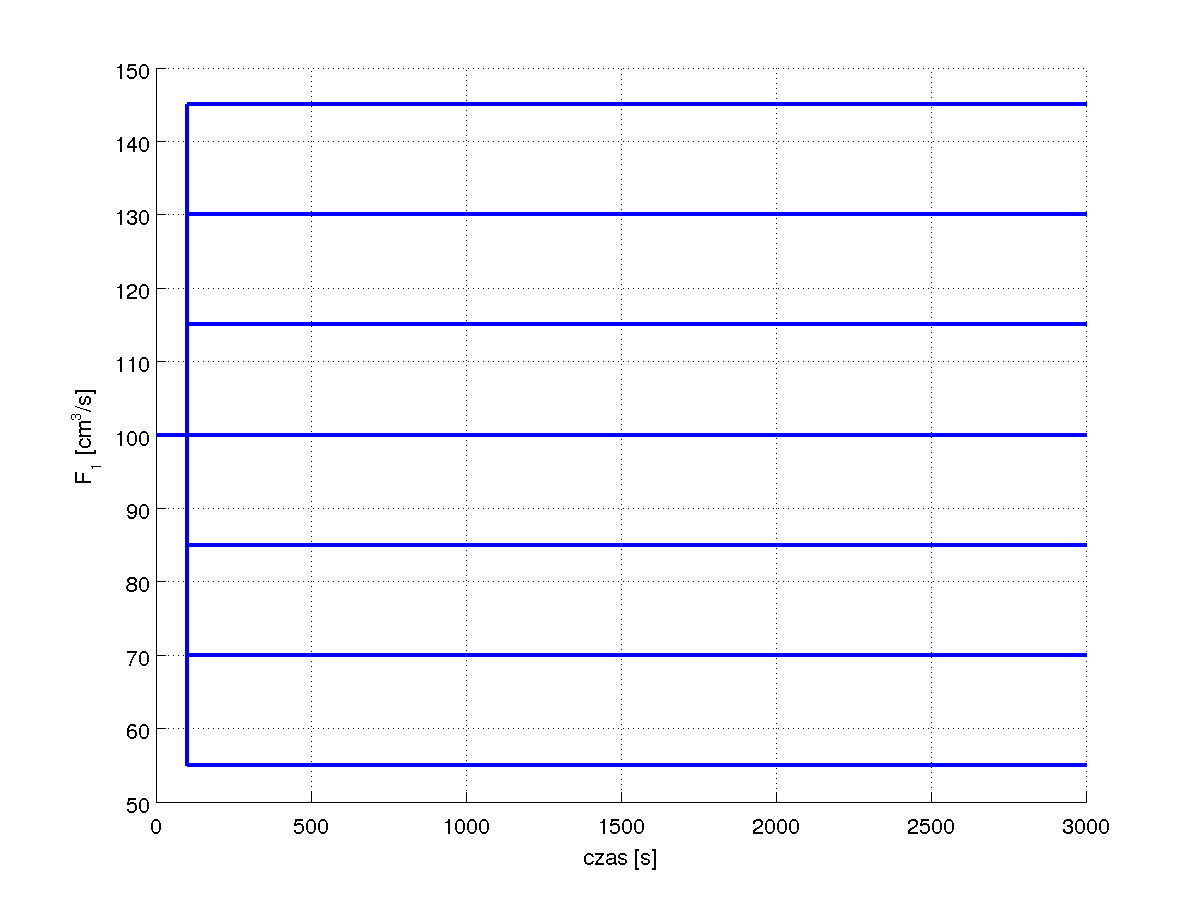
\includegraphics[width=\textwidth]{img/symulacja_z_liniowym_1a.png}
      \caption{Zmiany natężenia dopływającego strumienia sterującego.}
   \end{subfigure}
   \begin{subfigure}[h]{0.45\textwidth}
      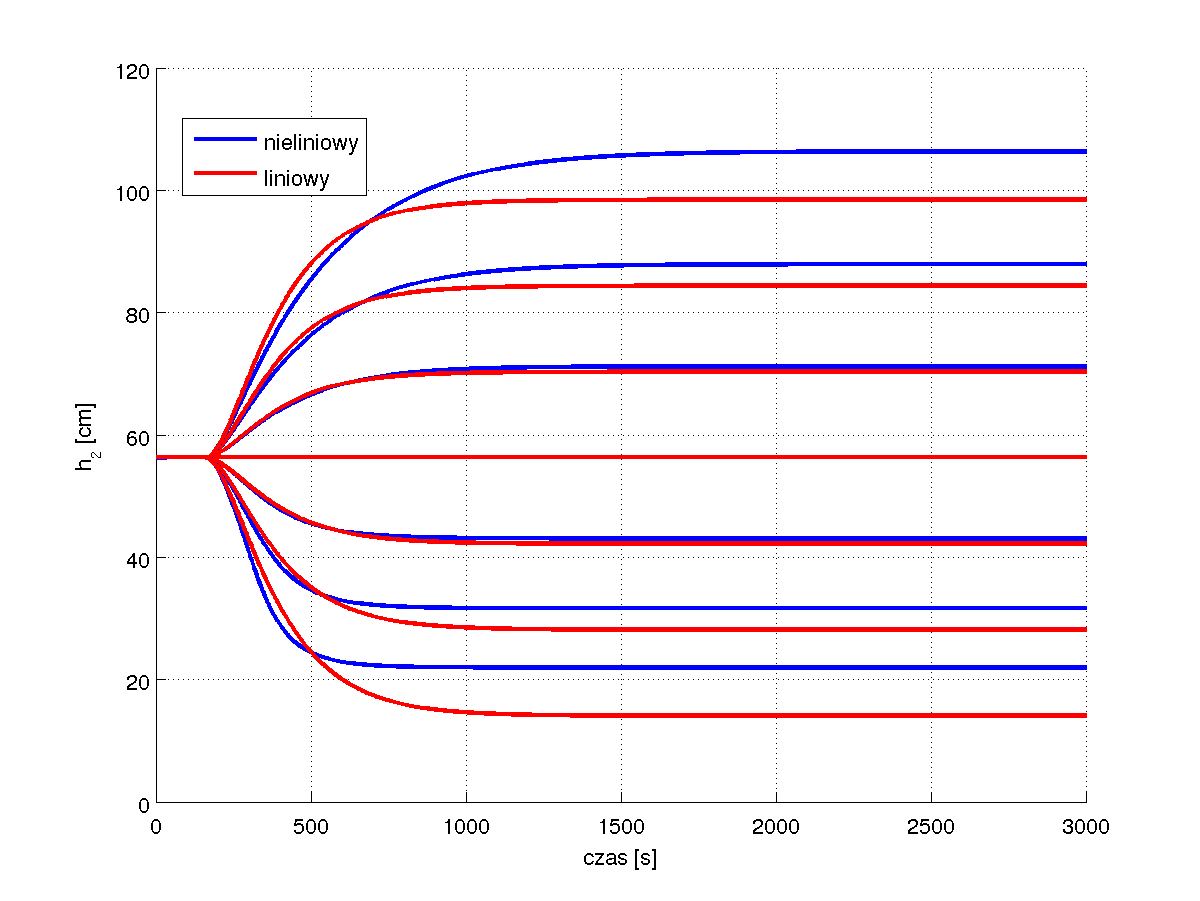
\includegraphics[width=\textwidth]{img/symulacja_z_liniowym_1b.png}
      \caption{Odpowiedzi obiektu na skok wartości na wejściu.}
   \end{subfigure}
   \caption{Porównanie modelu liniowego z oryginalnymi równaniami różniczkowymi obiektu.}
   \label{img:symulacja_z_liniowym}
\end{figure}

\paragraph{}
Rysunek \ref{img:symulacja_z_liniowym} przedstawia wynik symulacji modelu liniowego na tle oryginalnych równań różniczkowych obiektu.
Przy niewielkim oddalaniu się od punktu pracy model liniowy wciąż stosunkowo dokładnie oddaje zachowanie się obiektu, jednak przy znacznym oddaleniu się od punktu pracy nieliniowość obiektu jest coraz bardziej widoczna, a model liniowy coraz bardziej odbiega od rzeczywistości.

\newpage
\subsection{Liniowy model dyskretny}
\paragraph{}
Kolejnym celem zadania będzie sterowanie obiektem za pomocą algorytmu predykcyjnego GPC, dlatego model musi zostać przekształcony do postaci dyskretnego równania różnicowego.
Ponieważ obiekt jest dość wolny, przyjęty został dłuższy okres próbkowania: $T_p=5s$.
Model dyskretny został uzyskany za pośrednictwem narzędzi wbudowanych Matlaba, tj. zestawu funkcji \texttt{ss2tf} i \texttt{c2d}.
Wykorzystana została metoda dyskretyzacji bazująca na ekstrapolatorze zerowego rzędu.
Uzyskane równanie różnicowe (o przybliżonych wartościach numerycznych współczynników) jest następujące:

\begin{equation}
   \begin{array}{lcl}
   y(k) & = & 1.913202047891722 \cdot y(k-1) - 0.914885618196487 \cdot y(k-2) + \\[0.1cm]
   ~ & ~ & 0.000800873041280923 \cdot u(k-13) + 0.000777474119435667 \cdot u(k-14)
   \end{array}
\end{equation}

\noindent Wyniki tak uzyskanego modeu dyskretnego zostały przedstawione na tle równań różniczkowych obiektu i ciągłego modelu liniowego na wykresie \ref{img:symulacja_z_dyskretnym}.

\begin{figure}[h]
   \centering
   \begin{subfigure}[h]{0.45\textwidth}
      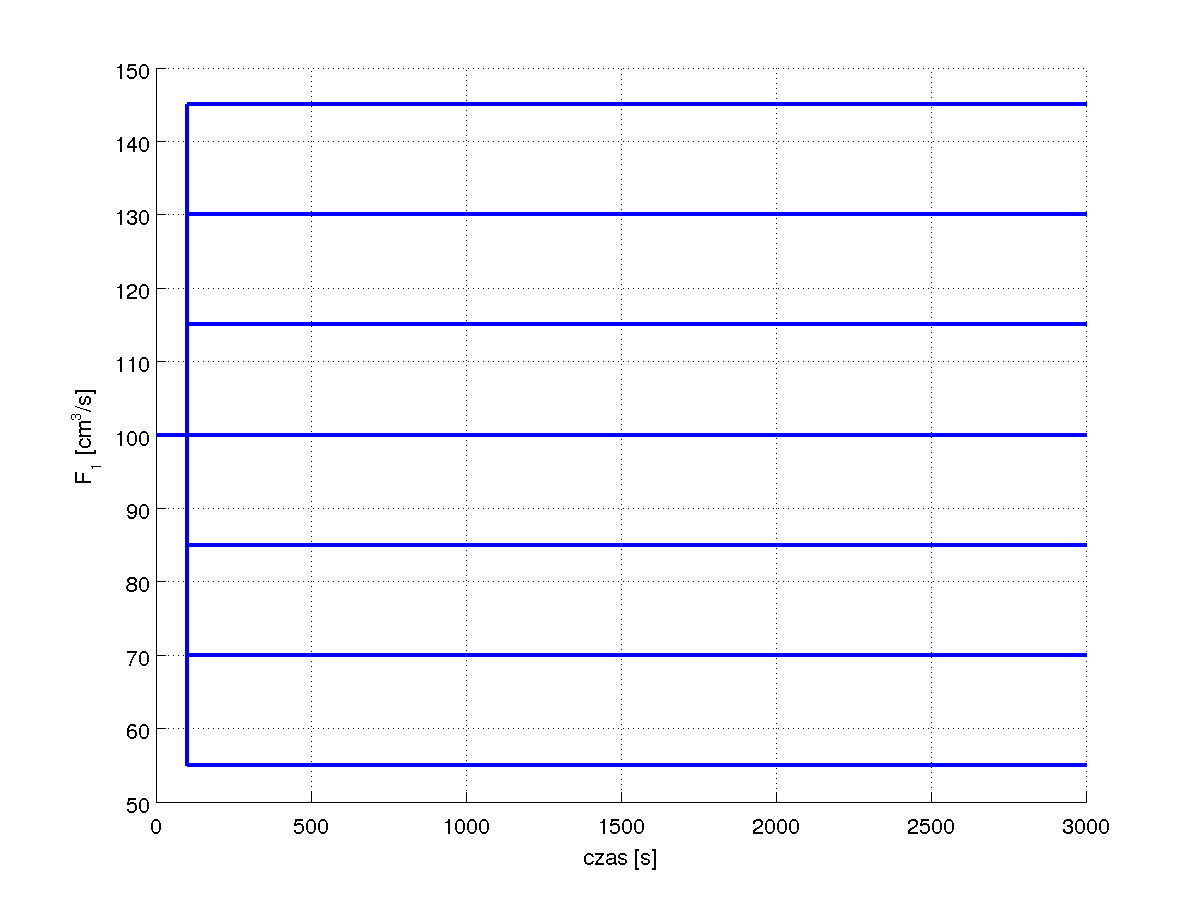
\includegraphics[width=\textwidth]{img/symulacja_z_dyskretnym_1a.png}
      \caption{Zmiany natężenia dopływającego strumienia sterującego.}
   \end{subfigure}
   \begin{subfigure}[h]{0.45\textwidth}
      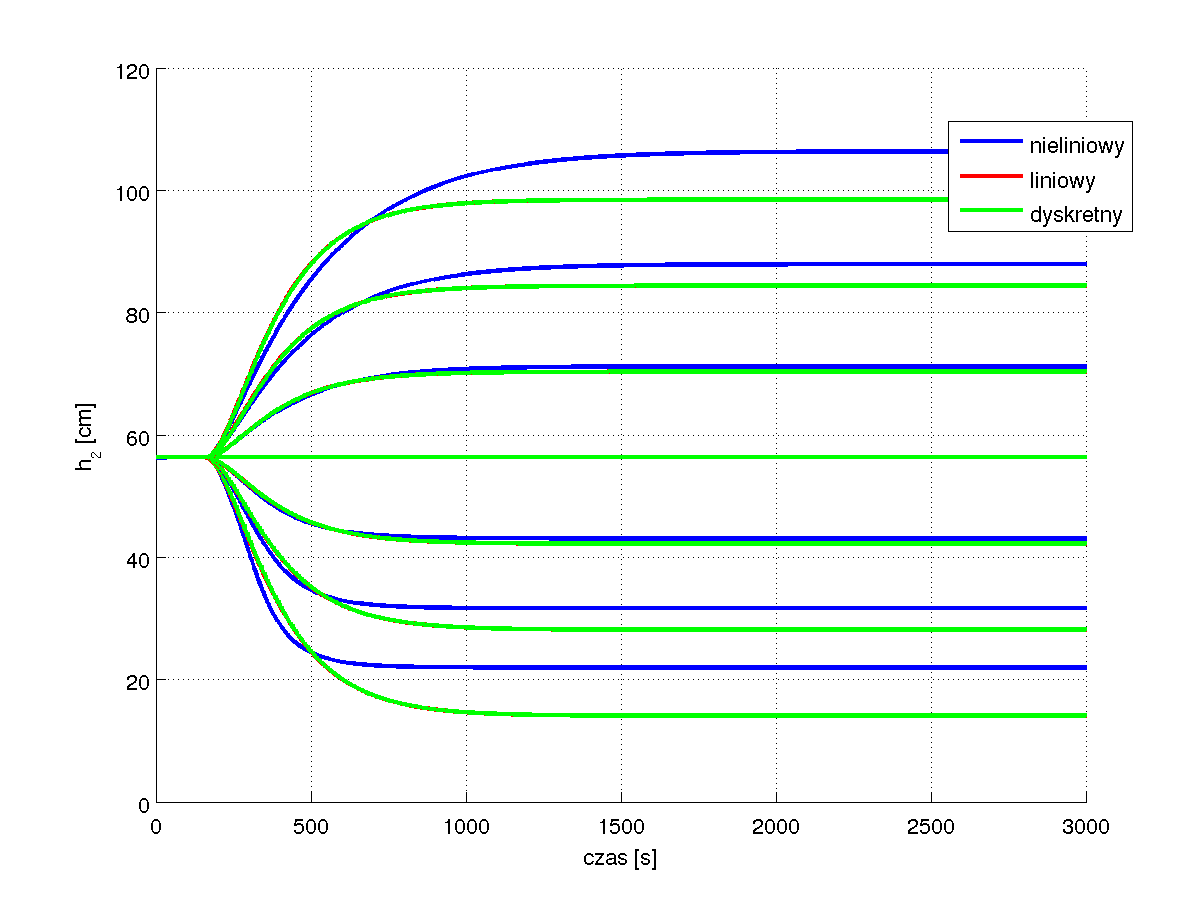
\includegraphics[width=\textwidth]{img/symulacja_z_dyskretnym_1b.png}
      \caption{Odpowiedzi obiektu na skok wartości na wejściu.}
   \end{subfigure}
   \caption{Porównanie modelu dyskretnego z liniowym ciągłym i oryginalnymi równaniami różniczkowymi obiektu.}
   \label{img:symulacja_z_dyskretnym}
\end{figure}

\subsection{Model rozmyty typu Takagi-Sugeno}
\paragraph{}
Jednym z podejść do tworzenia modeli nieliniowych jest koncepcja modeli rozmytych Takagi-Sugeno.
Regulatory oparte o modele rozmyte okazują się silnym narzędziem, zwłaszcza w aplikacjach, gdzie trudno jest uzyskać pełny, analityczny opis obiektu sterowanego.
W modelach rozmytych określa się stopień przynależności elementu $x$ do zbiorów rozmytych.
W przeciwieństwie do podejścia klasycznego, w którym element należał do jakiegoś zbioru lub nie (przynależność ostra), tutaj element może należeć do kilku zbiorów jednocześnie w sposób określony funkcją przynależności.
Zmienna pośrednia między zmienną numeryczną a zmienną symboliczną określana jest mianem \emph{zmiennej lingwistycznej}.

\paragraph{}
Modele rozmyte typu Takagi-Sugeno charakteryzują się regułami z następnikami funkcyjnymi, z których najczęściej wykorzystuje się wielomiany pierwszego rzędu.
Dzięki takiej postaci można w całkiem dokładny sposób modelować obiekt wykorzystując niewielki zbiór reguł.
Ponadto dodatkowe korzyści płyną z faktu, że istnieje szereg metod identyfikacji i konstrukcji modeli liniowych, co pozwala w stosunkowo łatwy sposób stworzyć model rozmyty, który z powodzeniem można wykorzystać w regulatorze.

\paragraph{}
W pracy przyjęty został zakres zmian wartości sterowania $F_1 \in <50,~150>$, wobec tego przyjętych zostało pięć modeli lokalnych, ulokowanych w punktach odpowiadających wartościom sterowania $F_1 \in \lbrace 50,~75,~100,~125,~150 \rbrace$.
Zmienną lingwistyczną jest poprzednie wyjście obiektu, czyli $y(k-1)$.
Ulokowanie modeli lokalnych wraz z ich wzmocnieniami przedstawiono na tle charakterystyki statycznej obiektu na rysunku \ref{img:lokalne_modele_liniowe}.

\begin{figure}[h]
   \centering
   \begin{subfigure}[h]{0.45\textwidth}
      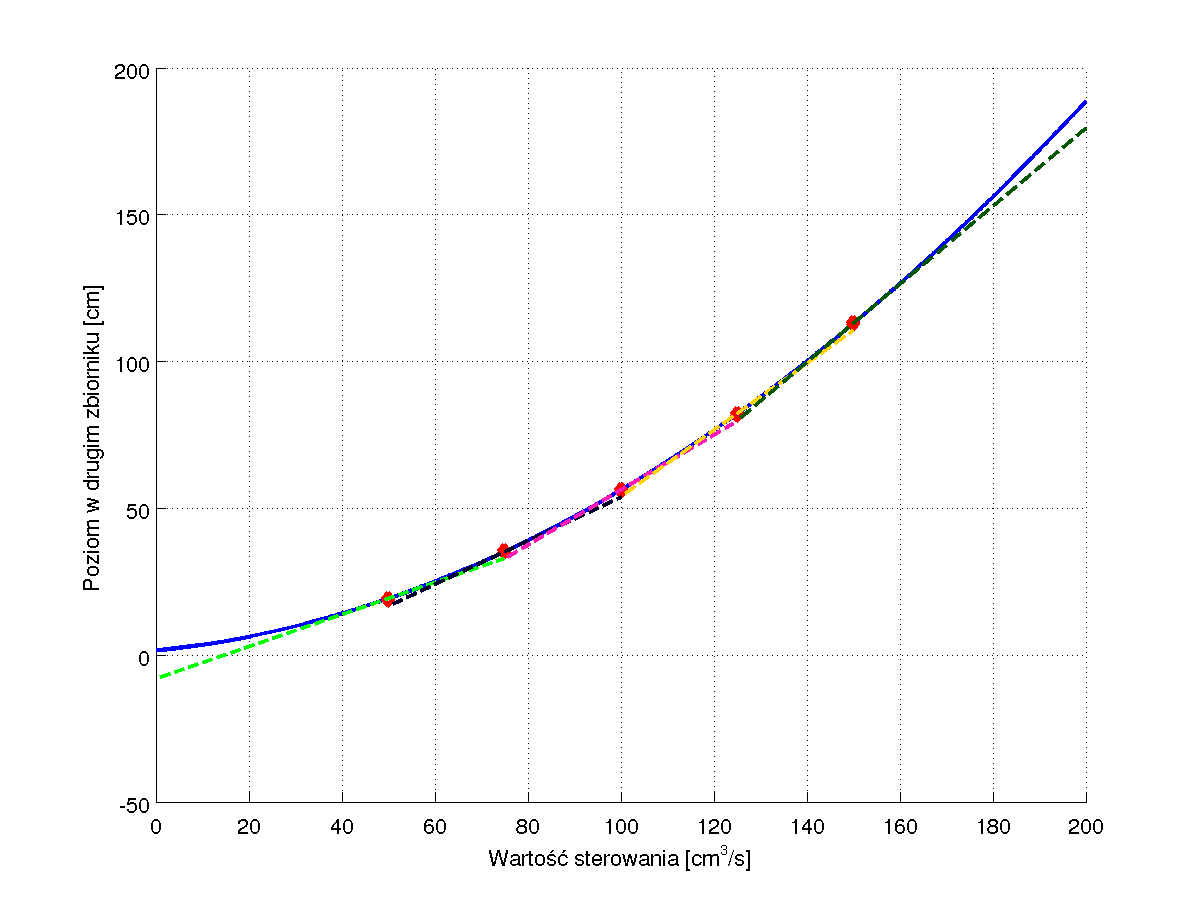
\includegraphics[width=\textwidth]{img/lokalne_modele_liniowe.png}
   \end{subfigure}
   \caption{Charakterystyka statyczna obiektu wraz z charakterystykami modeli lokalnych modelu rozmytego.}
   \label{img:lokalne_modele_liniowe}
\end{figure}

\paragraph{}
Początkowo funkcje przynależności zostały wybrane jako proste funkcje trapezowe i trójkątne.
Ich postaci przedstawia rysunek \ref{img:trapezoid_mfs}.
Wzory funkcji zostały dopasowane tak, aby modele lokalne przełączane były w sposób liniowy, wartość 1 jest osiągana w punkcie pracy modelu lokalnego.
W ten sposób co najwyżej dwa modele lokalne są aktywne jednocześnie.

\newpage

\begin{figure}[h]
   \centering
   \begin{subfigure}[h]{0.45\textwidth}
      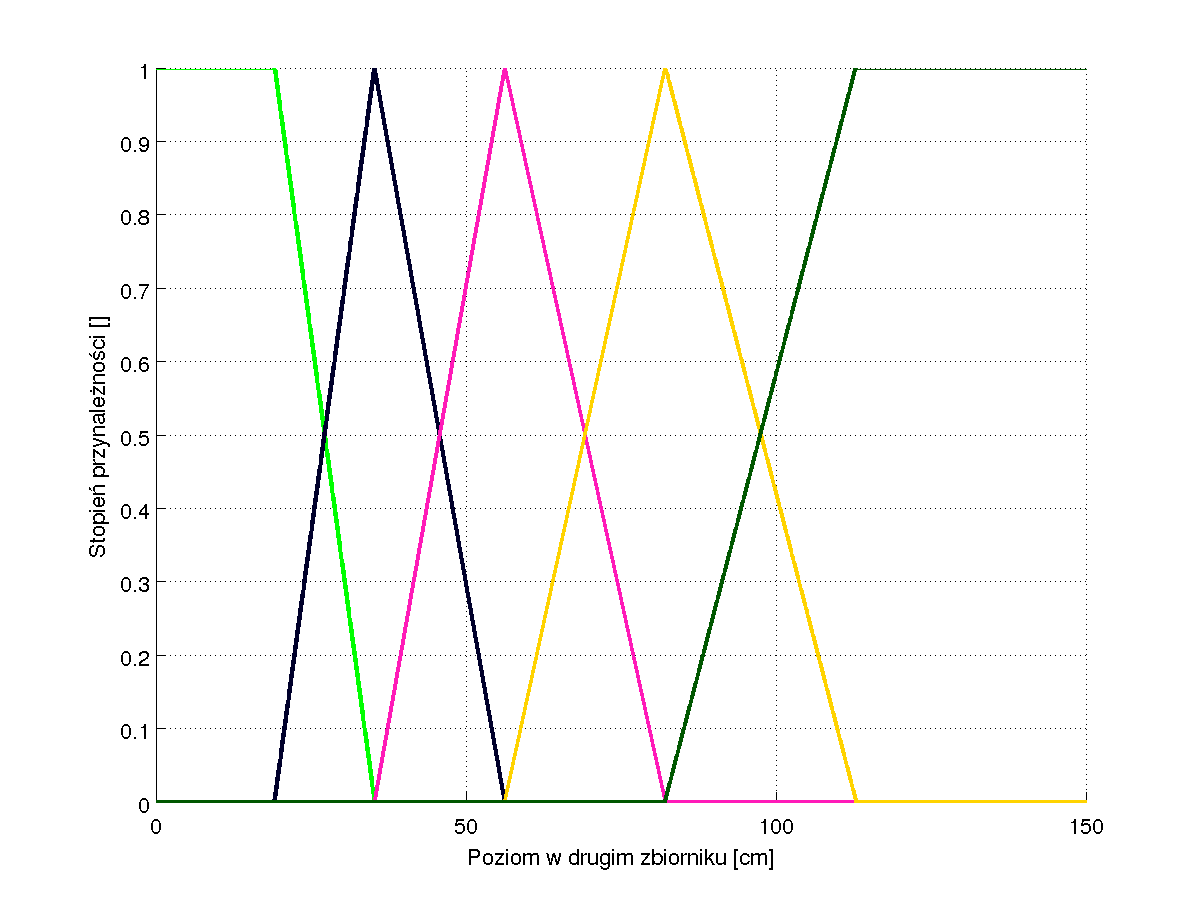
\includegraphics[width=\textwidth]{img/trapezoid_mfs.png}
   \end{subfigure}
   \caption{Funkcje przynależności wstępnego modelu rozmytego.}
   \label{img:trapezoid_mfs}
\end{figure}

\paragraph{}
Wyniki symulacji modelu rozmytego zostały przedstawione na tle modelu liniowego i rzeczywistych danych obiektu na rysunku \ref{img:modele_1}.
W modelu rozmytym wykorzystywane są informacje z innych obszarów, stąd występują zdecydowanie mniejsze uchyby ustalone w porównaniu z modelem liniowym.
Ponadto zmienna jest także dynamika modelu rozmytego, stąd model rozmyty lepiej odwzorowuje obiekt rzeczywisty.
Dopasowanie tak uzyskanego modelu rozmytego do obiektu w zakładanym przedziale działania powinno być wystarczające do wykorzystania w syntezie regulatorów rozmytych.

\begin{figure}[h]
   \centering
   \begin{subfigure}[h]{0.45\textwidth}
      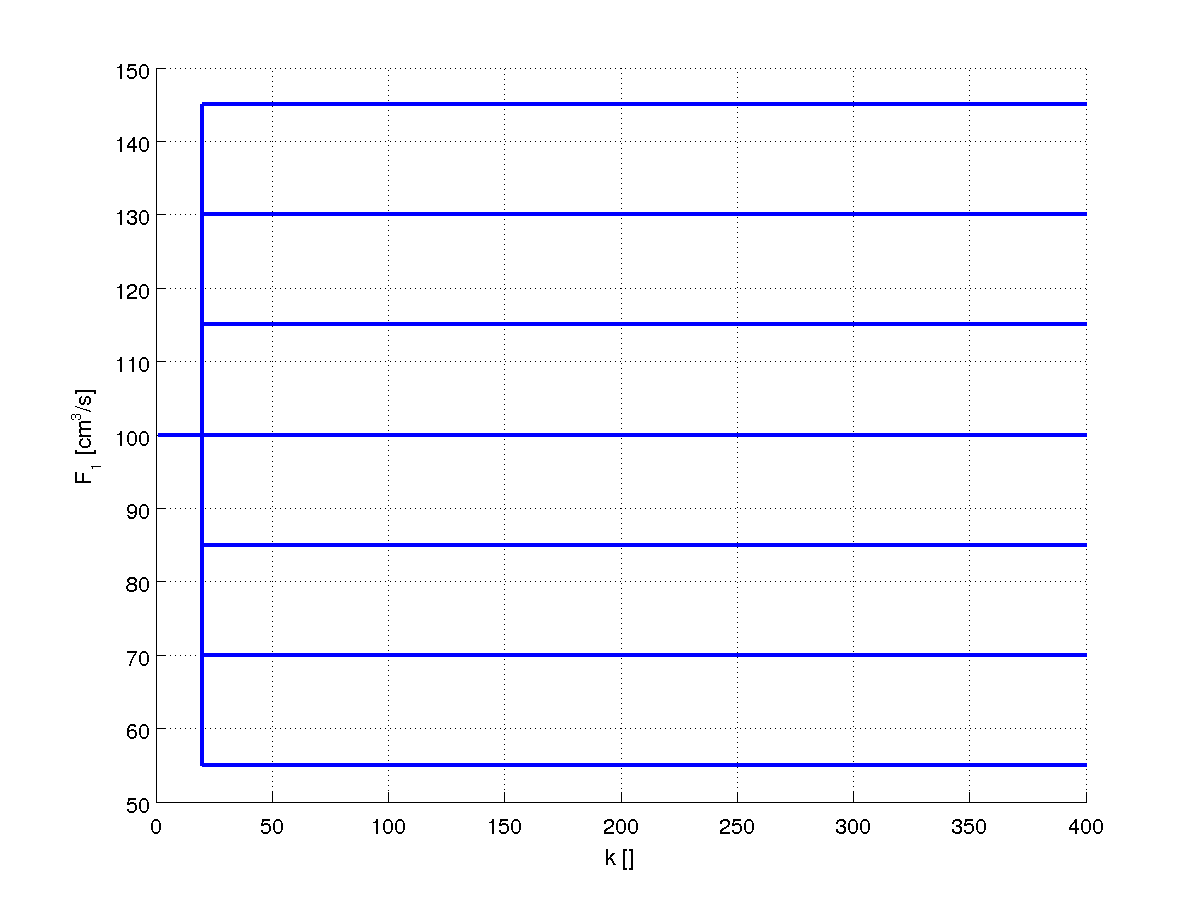
\includegraphics[width=\textwidth]{img/modele_1a.png}
      \caption{Zmiany natężenia dopływającego strumienia sterującego.}
   \end{subfigure}
   \begin{subfigure}[h]{0.45\textwidth}
      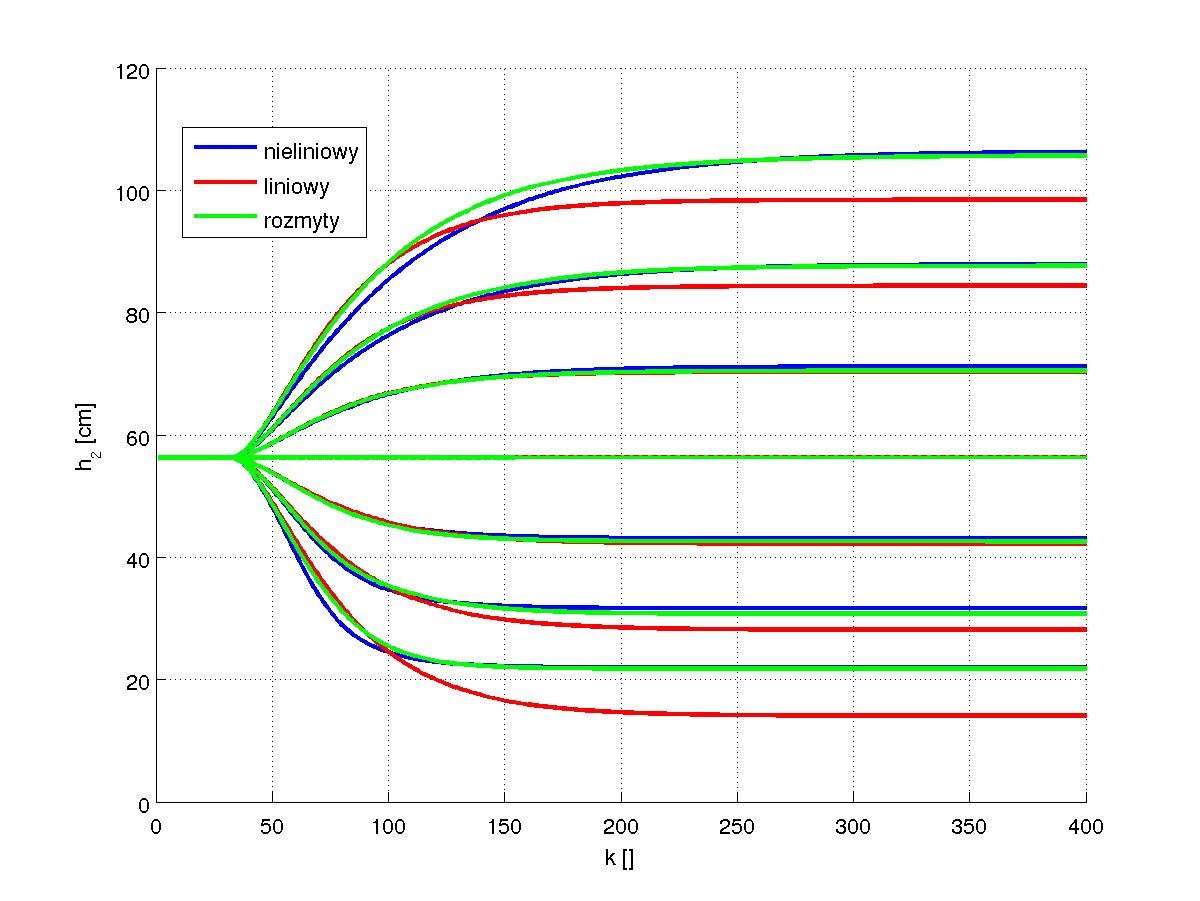
\includegraphics[width=\textwidth]{img/modele_1b.png}
      \caption{Odpowiedzi obiektu i modeli na skok wartości na wejściu.}
   \end{subfigure}
   \caption{Porównanie modelu rozmytego z liniowym dyskretnym i oryginalnymi równaniami różniczkowymi obiektu.}
   \label{img:modele_1}
\end{figure}

\newpage

\subsection{Strojenie parametrów modelu rozmytego.}
\paragraph{}
Warto sprawdzić, czy sposób przełączania modeli lokalnych może zostać poprawiony stosując inny kształt funkcji przynależności.
Do tego celu zastosowano funkcje dzwonowe, które opisane są wzorem:

\begin{equation}
   \mu(x) ~=~ \frac{1}{1 + \left|\frac{x-c}{b}\right|^{2a}}
\end{equation}

\noindent w której parametr $c$ odpowiada za środek symetrii dzwonu, a parametry $a$ i $b$ za kształt funkcji.
Dzwonowe funkcje przynależności zostały dopasowane do przebiegów trójkątnych i prostokątnych za pomocą narzędzia \texttt{cftool} programu Matlab.
Rysunek \ref{img:mfs} przedstawia porównanie zbiorów funkcji przynależności trójkątnych do dzwonowych.
Warto wspomnieć, że model rozmyty w wersji z dzwonowymi funkcjami przynależności dalej dysponuje tymi samymi modelami lokalnymi.

\begin{figure}[h]
   \centering
   \begin{subfigure}[h]{0.45\textwidth}
      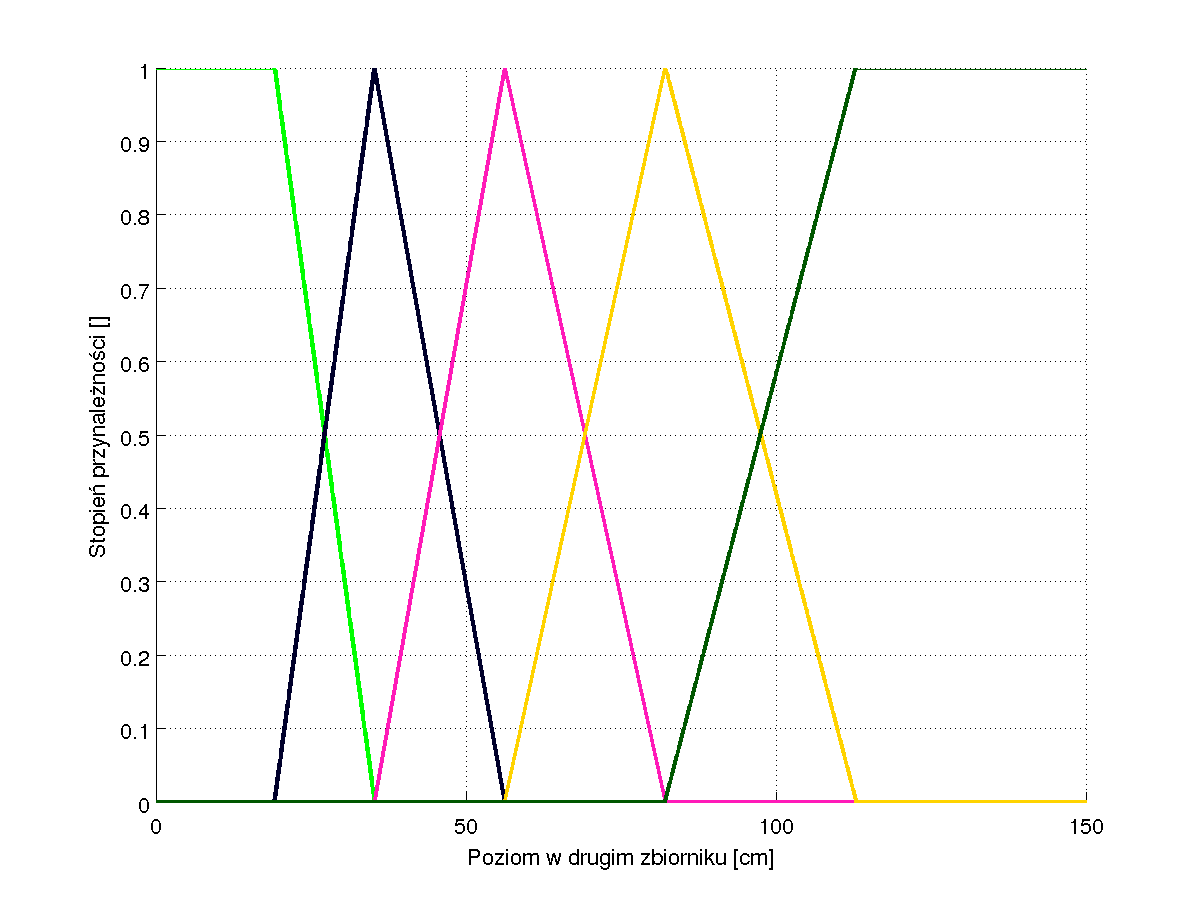
\includegraphics[width=\textwidth]{img/trapezoid_mfs.png}
      \caption{Trapezowe i trójkątne funkcje przynależności.}
   \end{subfigure}
   \begin{subfigure}[h]{0.45\textwidth}
      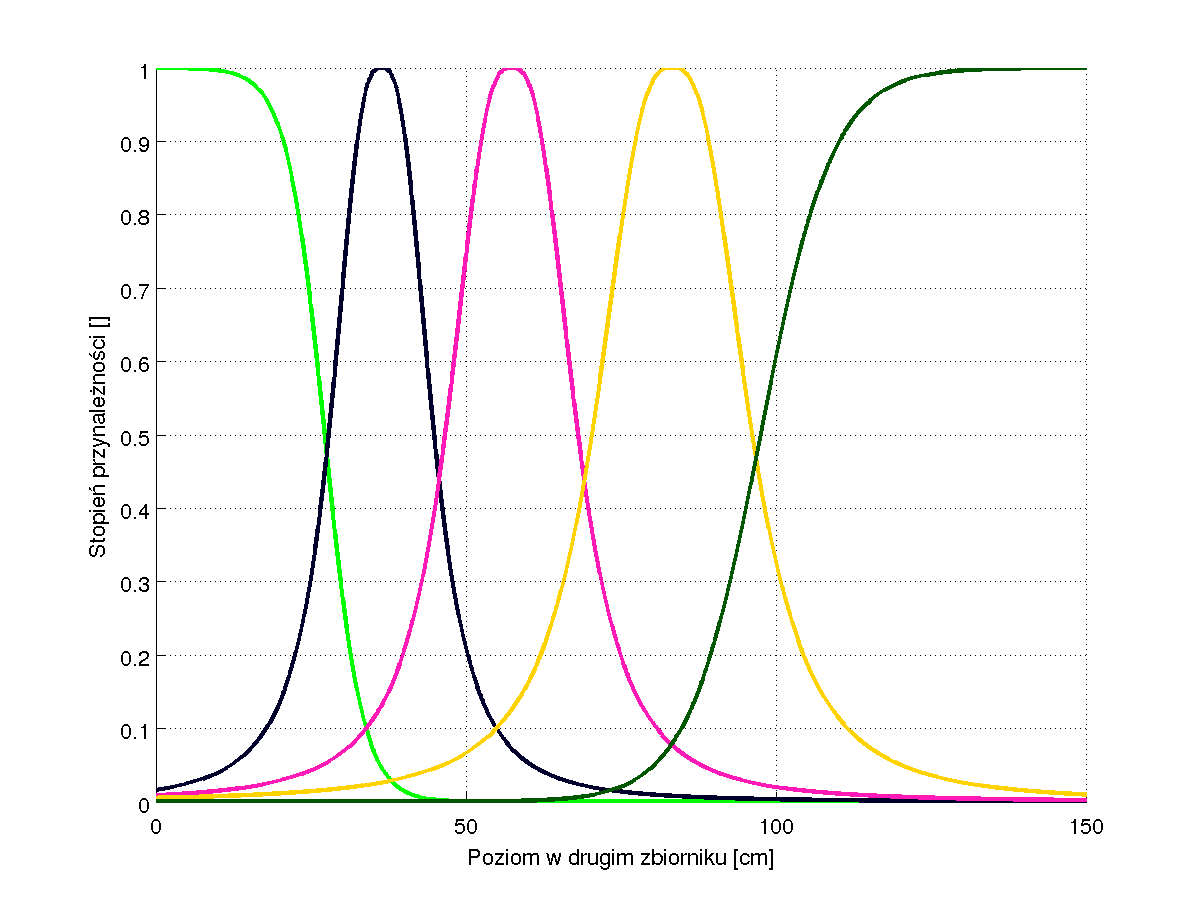
\includegraphics[width=\textwidth]{img/mfs_1b.png}
      \caption{Dzwonowe funkcje przynależności.}
   \end{subfigure}
   \caption{Porównanie dwóch zestawów funkcji przynależności o innych kształtach.}
   \label{img:mfs}
\end{figure}

\paragraph{}
Kryterium jakości zadania optymalizacji stanowiła suma kwadratów błędów na wygenerowanej trajektorii wyjścia obiektu, gdzie przez błąd rozumiana była różnica pomiędzy wyjściem z obiektu i wyjściem z modelu rozmytego.
Wektor zmiennych decyzyjnych zbudowany był z parametrów wszystkich kolejnych funkcji przynależności, a ograniczenia na zmienne decyzyjne zostały nałożone w następujący sposób:

\begin{equation}
   \begin{gathered}
      LB ~=~ \left[ \text{min} \lbrace0.8a^i,~1.2a^i\rbrace;~\text{min}\lbrace0.8b^i,~1.2b^i\rbrace;~\text{min}\lbrace0.9c^i,~1.1c^i\rbrace \right],~~i=1,...5\\[0.2cm]
      UB ~=~ \left[ \text{max} \lbrace0.8a^i,~1.2a^i\rbrace;~\text{max}\lbrace0.8b^i,~1.2b^i\rbrace;~\text{max}\lbrace0.9c^i,~1.1c^i\rbrace \right],~~i=1,...5
   \end{gathered}
\end{equation}

\newpage
\noindent Wynikowe kształty funkcji przynależności po optymalizacji parametrów są przedstawione na rysunku \ref{img:optimized_mfs}. Krzywe dzwonowe uległy zarówno przesunięciom, jak i zmienił się ich kształt. 
Trajektorie wyjść obiektu i wyjść obydwu modeli rozmytych (wykorzystującego startowe postaci funkcji dzwonowych i postaci po optymalizacji) są przedstawione na rysunku \ref{img:trajectories}.
Można zauważyć, że przebieg wyjścia z modelu zoptymalizowanego nie zmienił się znacznie w porównaniu do modelu z początkowymi wartościami parametrów.

\begin{figure}[h]
   \centering
   \begin{subfigure}[h]{0.45\textwidth}
      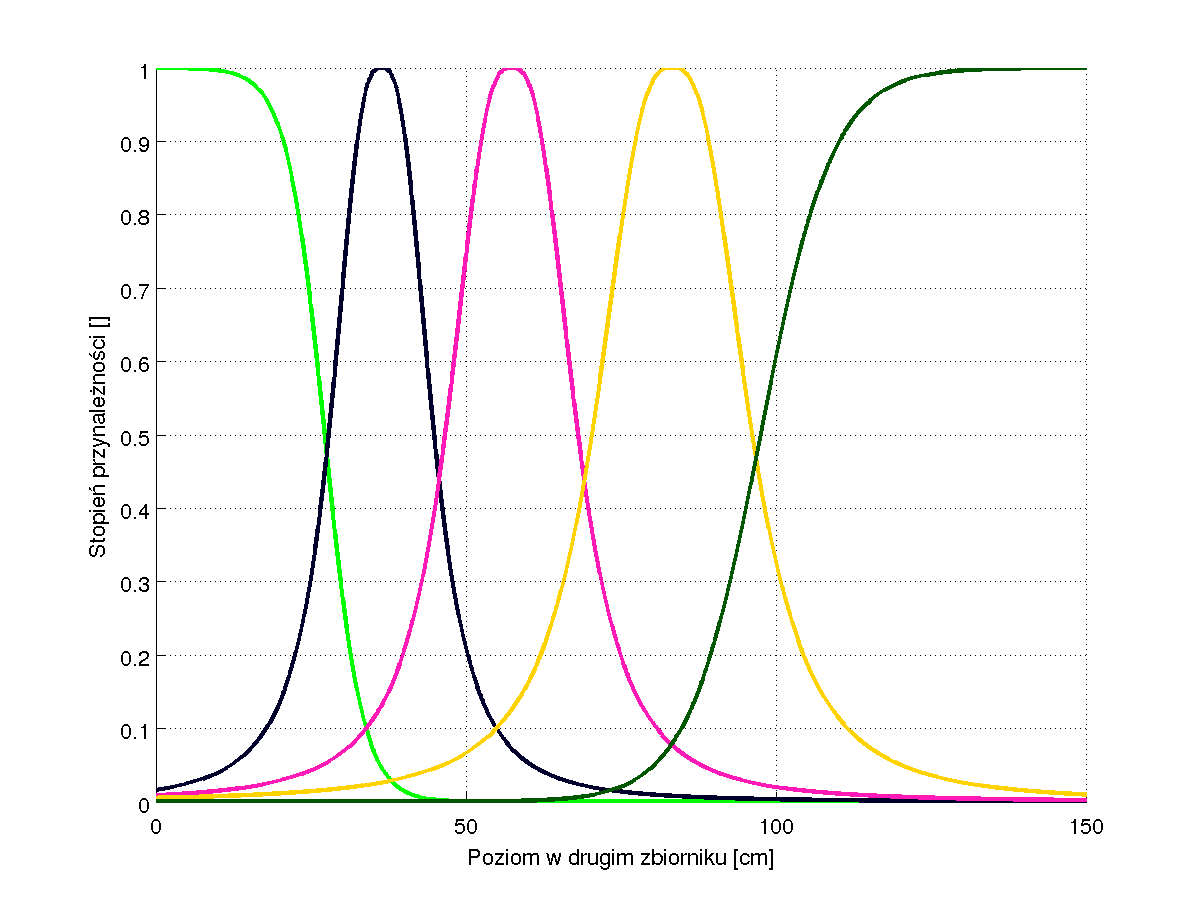
\includegraphics[width=\textwidth]{img/optimization_mfs_1.png}
      \caption{Funkcje przynależności przed optymalizacją.}
   \end{subfigure}
   \\
   \begin{subfigure}[h]{0.45\textwidth}
      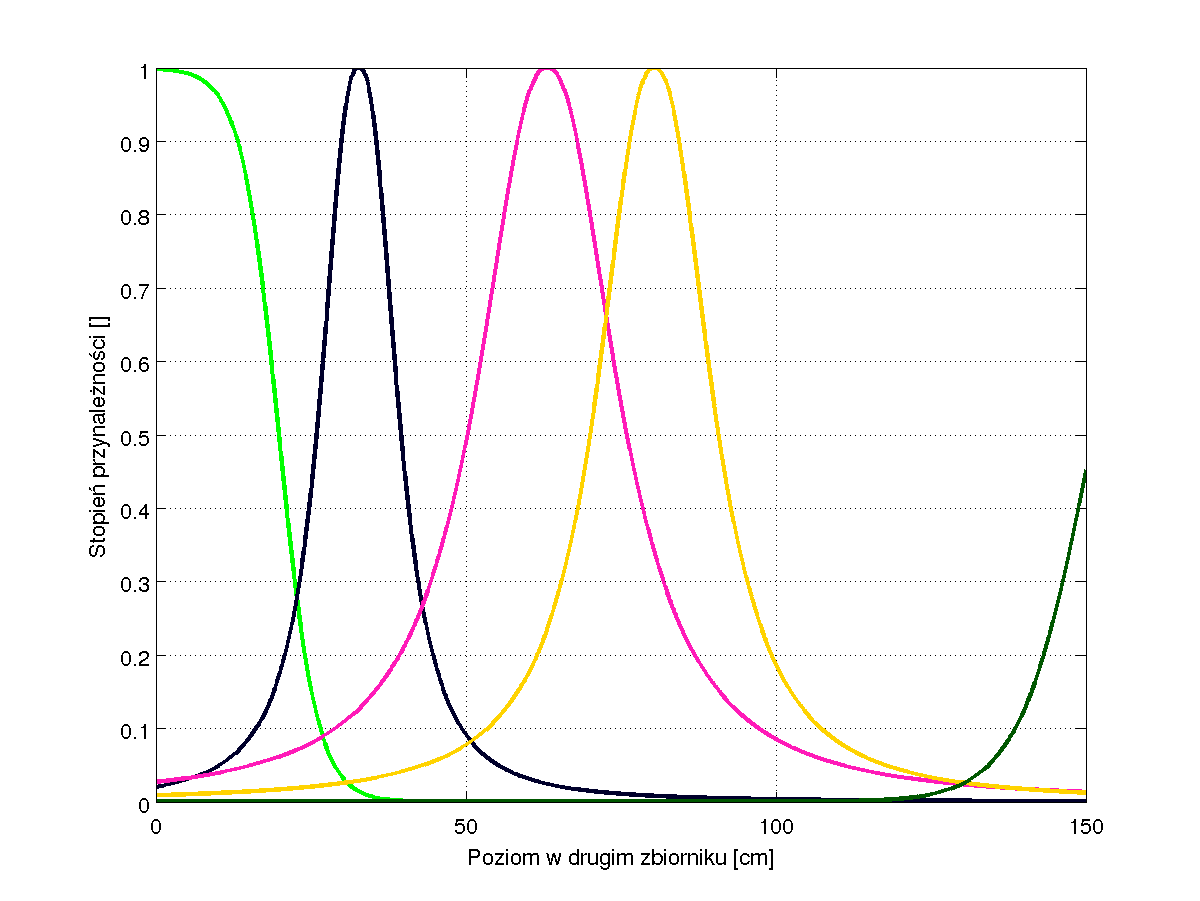
\includegraphics[width=\textwidth]{img/optimization_mfs_2.png}
      \caption{Funkcje przynależności po optymalizacji.}
   \end{subfigure}
   \caption{Porównanie zestawów funkcji przynależności po optymalizacji.}
   \label{img:optimized_mfs}
\end{figure}

\newpage
\begin{figure}[h]
   \centering
   \begin{subfigure}[h]{0.45\textwidth}
      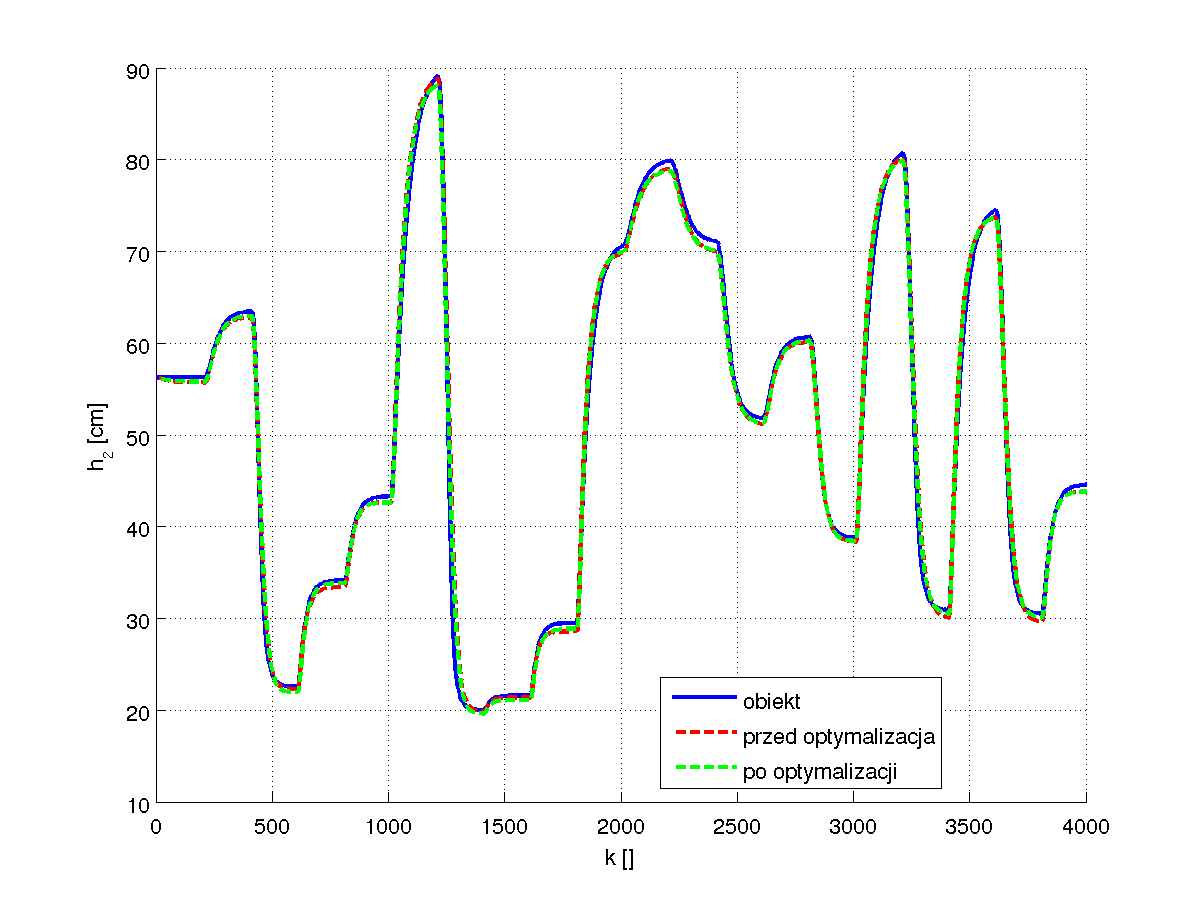
\includegraphics[width=\textwidth]{img/trajectories.png}
   \end{subfigure}
   \caption{Porównanie zestawów funkcji przynależności po optymalizacji.}
   \label{img:trajectories}
\end{figure}

\paragraph{}
Ostatnim testem było porównanie wszystkich trzech modeli rozmytych:
\begin{itemize}
   \item wykorzystującego trójkątne i trapezowe funkcje przynależności;
   \item wykorzystującego dzwonowe funkcje przynależności;
   \item wykorzystującego dzwonowe funkcje przynależności, po optymalizacji ich parametrów.
\end{itemize}
\noindent Symulacja zachowania wszystkich modeli na skoki wartości wejściowej przedstawiono na rysunku \ref{img:fuzzy_comparison}.
Najbardziej wyraźną różnicę w działaniu można zaobserwować dla największej wielkości skoku.
Najlepiej odwzorowuje obiekt model oparty na trapezowych funkcjach przynależności i ten model zostanie wykorzystany do syntezy regulatorów rozmytych.

\begin{figure}[h]
   \centering
   \begin{subfigure}[h]{0.45\textwidth}
      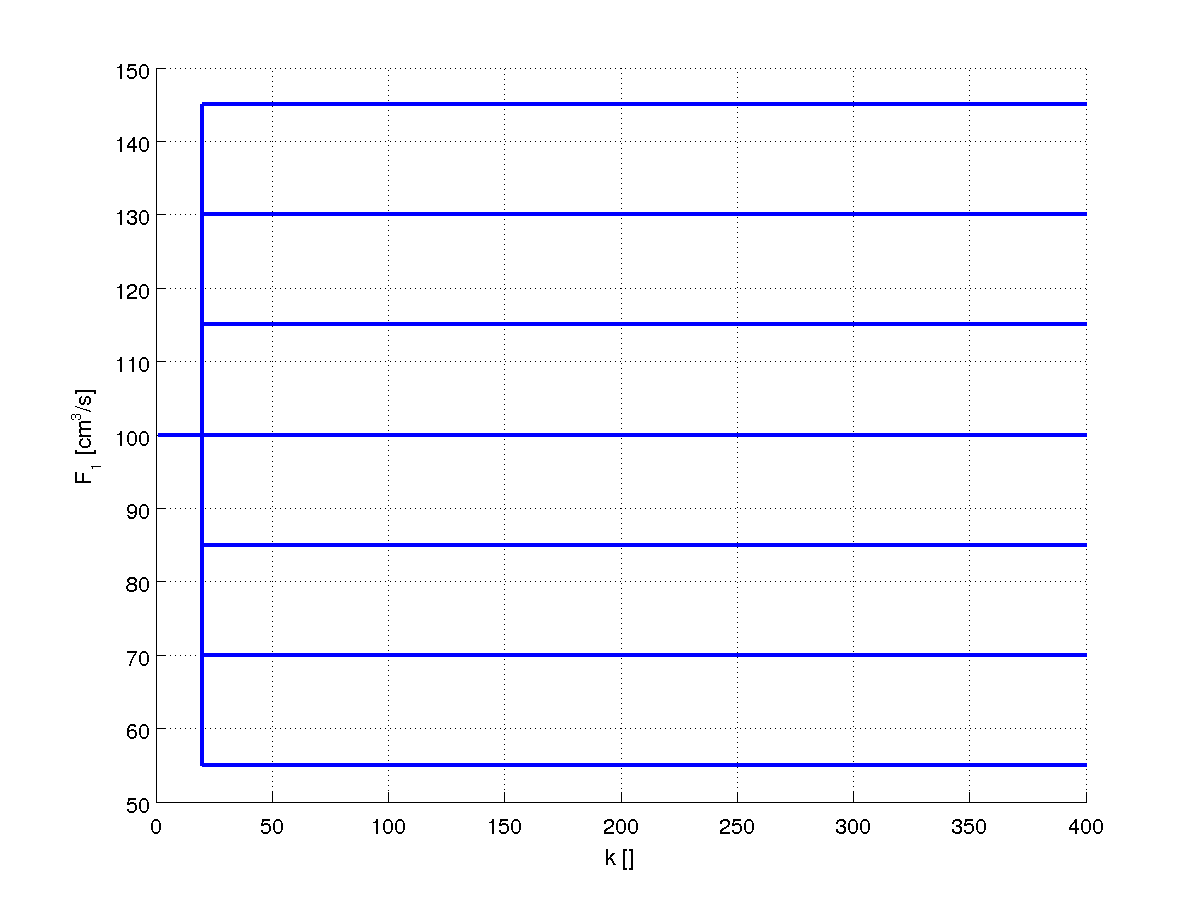
\includegraphics[width=\textwidth]{img/fuzzy_comparison_1a.png}
      \caption{Skoki wartości podane na wejścia obiektu.}
   \end{subfigure}
   \begin{subfigure}[h]{0.45\textwidth}
      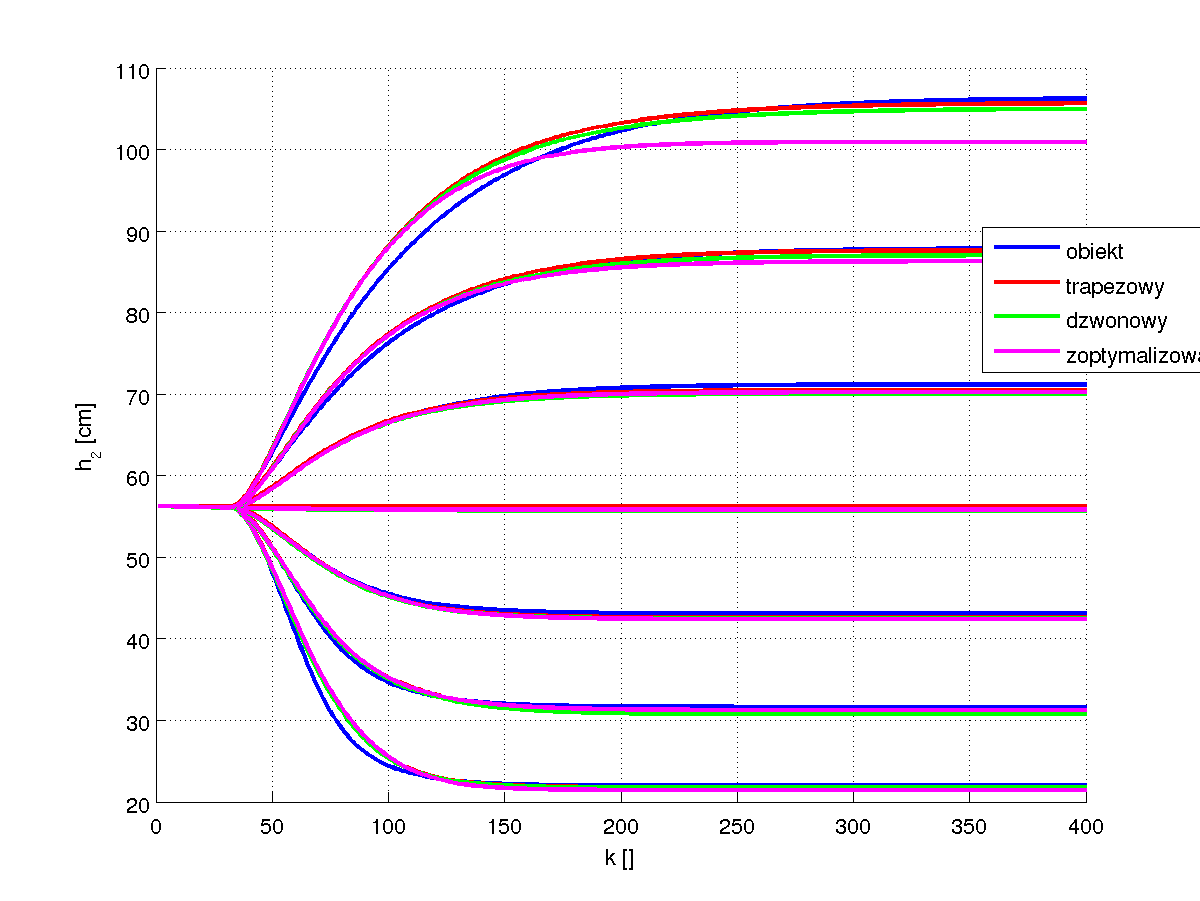
\includegraphics[width=\textwidth]{img/fuzzy_comparison_1b.png}
      \caption{Odpowiedzi obiektu i modeli.}
   \end{subfigure}
   \caption{Porównanie modeli rozmytych.}
   \label{img:fuzzy_comparison}
\end{figure}



% \paragraph{}
% Należy jeszcze zaznaczyć w jaki sposób wyjście obiektu zależy od równań opisujących stan obiektu.
% Wyjściem zostaną nazwane wartości regulowane, to jest wysokość poziomu wody w zbiorniku i temperatura wypływającej wody.
% Kwestia opóźnień na wejściu i wyjściu obiektu zostanie na chwilę obecną pominięta ze względu na trudność modelowania opóźnień w postaci równań stanu.
% Tworzony model pozostaje adekwatny do obiektu pod założeniem, że wejścia i wyjścia modelu będą w odpowiedni sposób opóźniane poza nim.
% Pod tymi założeniami jedno z wyjść jest wprost wartością temperatury wody wewnątrz obiektu.
% 
% \paragraph{}
% Dane równanie opisujące zależność objętości wody od wysokości poziomu wody zostało przekształcone tak, aby wyrazić odwrotną zależność:
% 
% \begin{equation}
%    h ~=~ \begin{matrix}\sqrt[3]{\frac{1}{C}}\end{matrix} \cdot \sqrt[3]{V}
% \end{equation}
% 
% \paragraph{}
% Po przekształceniach równań obiektu można zdefiniować je jako funkcje:
% 
% \begin{equation}
%    \begin{array}{lllll}
%       f_1(F_H,F_C,F_D,V) &=& \begin{matrix}\frac{\text{d}V}{\text{d}t}\end{matrix} & = & F_H ~+~ F_C ~+~ F_D ~-~ \alpha\sqrt[6]{\begin{matrix}\frac{1}{C}\end{matrix}}\sqrt[6]{V}\\[0.2cm]
%       f_2(F_H,F_C,F_D,T_D,V,T) &=& \begin{matrix}\frac{\text{d}T}{\text{d}t}\end{matrix} & = & T_H \cdot \begin{matrix}\frac{F_H}{V}\end{matrix} + T_C \cdot \begin{matrix}\frac{F_C}{V}\end{matrix} + T_D \cdot \begin{matrix}\frac{F_D}{V}\end{matrix} - T \cdot \begin{matrix}\frac{F_H+F_C+F_D}{V}\end{matrix}
%    \end{array}
% \end{equation}
% 
% \noindent a następnie obliczyć ich pochodne czątkowe po każdej ze zmiennych.
% Tak więc pochodne cząstkowe funkcji $f_1$ wynoszą:
% 
% \begin{equation}
%    \begin{gathered}
%       \begin{matrix}\frac{\partial f_1}{\partial F_H}\end{matrix} ~=~ 1\\[0.1cm]
%       \begin{matrix}\frac{\partial f_1}{\partial F_C}\end{matrix} ~=~ 1\\[0.1cm]
%       \begin{matrix}\frac{\partial f_1}{\partial F_D}\end{matrix} ~=~ 1\\[0.1cm]
%       \begin{matrix}\frac{\partial f_1}{\partial V}\end{matrix} ~=~ - \begin{matrix}\frac{1}{6}\end{matrix} \cdot \alpha \cdot \sqrt[6]{\begin{matrix}\frac{1}{C}\end{matrix}} \cdot V^{-\frac{5}{6}}\\[0.1cm]
%    \end{gathered}
% \end{equation}
% 
% \noindent a dla funkcji $f_2$ są one następujące:
% 
% \begin{equation}
%    \begin{gathered}
%       \begin{matrix}\frac{\partial f_2}{\partial F_H}\end{matrix} ~=~ \begin{matrix}\frac{T_H~-~T}{V}\end{matrix}\\[0.1cm]
%       \begin{matrix}\frac{\partial f_2}{\partial F_C}\end{matrix} ~=~ \begin{matrix}\frac{T_C~-~T}{V}\end{matrix}\\[0.1cm]
%       \begin{matrix}\frac{\partial f_2}{\partial F_D}\end{matrix} ~=~ \begin{matrix}\frac{T_D~-~T}{V}\end{matrix}\\[0.1cm]
%       \begin{matrix}\frac{\partial f_2}{\partial T_D}\end{matrix} ~=~ \begin{matrix}\frac{F_D}{V}\end{matrix}\\[0.1cm]
%       \begin{matrix}\frac{\partial f_2}{\partial V}\end{matrix} ~=~ \begin{matrix}\frac{T(F_H+F_C+F_D)~-~T_HF_H~-~T_CF_C~-~T_DF_D}{V^2}\end{matrix}\\[0.1cm]
%       \begin{matrix}\frac{\partial f_2}{\partial T}\end{matrix} ~=~ - \begin{matrix}\frac{F_H~+~F_C~+~F_D}{V}\end{matrix}\\
%    \end{gathered}
% \end{equation}
% 
% \noindent Ponadto warto także obliczyć pochodną funkcji wysokości po objętości wody w zbiorniku:
% 
% \begin{equation}
%    \begin{matrix}\frac{\partial h}{\partial V}\end{matrix} ~=~ \begin{matrix}\frac{1}{3}\end{matrix} \cdot \sqrt[3]{\begin{matrix}\frac{1}{C}\end{matrix}} \cdot V^{-\frac{2}{3}}
% \end{equation}
% 
% \paragraph{}
% Tak obliczone pochodne posłużą bezpośrednio do zapisania modelu liniowego w postaci równań stanu, muszą jednak zostać obliczone ich wartości w punkcie pracy.
% Należy pamiętać, że tak utworzony zlinearyzowany model odnosi się do zmian wartości wejść, stanów i wyjść w stosunku do wartości tych zmiennych w punkcie pracy.
% Ciągły model wyrażony za pomocą równań stanu jest więc postaci:
% 
% \begin{equation}
%    \begin{gathered}
%       \dot{\boldsymbol{x}} ~=~ \boldsymbol{Ax} + \boldsymbol{Bu}\\[0.1cm]
%       \boldsymbol{y} ~=~ \boldsymbol{Cx} + \boldsymbol{Du}
%    \end{gathered}
% \end{equation}
% 
% \noindent gdzie:
% 
% \begin{equation}
%    \begin{gathered}
%       \boldsymbol{x} ~=~ \left[ 
%       \begin{array}{c}
%          V - V_0\\
%          T - T_0\\
%       \end{array}
%       \right],
%       ~~~~~~~~~~~~~
%       \boldsymbol{u} ~=~ \left[ 
%       \begin{array}{c}
%          F_H - F_{H0}\\
%          F_C - F_{C0}\\
%          F_D - F_{D0}\\
%          T_D - T_{D0}\\
%       \end{array}
%       \right]
%       \\%[0.2cm]
%       \boldsymbol{y} ~=~ \left[ 
%       \begin{array}{c}
%          h - h_0\\
%          T - T_0\\
%       \end{array}
%       \right]
%    \end{gathered}
% \end{equation}
% 
% \paragraph{}
% Macierze $\boldsymbol{A}, \boldsymbol{B}$ i $\boldsymbol{C}$ składają się więc z następujących elementów (dla uproszczenia zapisu przyjąłem oznaczenie $p.p.$ jako warunek zdefiniowany przez punkt pracy podany w treści polecenia):
% 
% \begin{equation}
%    \begin{gathered}
%       \boldsymbol{A} ~=~
%       \left[
%          \begin{array}{cc}
%             \left. \frac{\partial f_1}{\partial V} \right|_{p.p.} & 
%                \left. \frac{\partial f_1}{\partial T} \right|_{p.p.}\\[0.2cm]
%             \left. \frac{\partial f_2}{\partial V} \right|_{p.p.} & 
%                \left. \frac{\partial f_2}{\partial T} \right|_{p.p.}
%          \end{array}
%       \right]\\[0.2cm]
%       \boldsymbol{B} ~=~
%       \left[
%          \begin{array}{cccc}
%             \left. \frac{\partial f_1}{\partial F_H} \right|_{p.p.} & 
%                 \left. \frac{\partial f_1}{\partial F_C} \right|_{p.p.} &
%                 \left. \frac{\partial f_1}{\partial F_D} \right|_{p.p.} &
%                 \left. \frac{\partial f_1}{\partial T_D} \right|_{p.p.} \\[0.2cm]
%             \left. \frac{\partial f_2}{\partial F_H} \right|_{p.p.} & 
%                 \left. \frac{\partial f_2}{\partial F_C} \right|_{p.p.} &
%                 \left. \frac{\partial f_2}{\partial F_D} \right|_{p.p.} &
%                 \left. \frac{\partial f_2}{\partial T_D} \right|_{p.p.}
%          \end{array}
%       \right]\\[0.2cm]
%       \boldsymbol{C} ~=~
%       \left[
%          \begin{array}{cc}
%             \left. \frac{\partial h}{\partial V} \right|_{p.p.} & 
%                \left. \frac{\partial h}{\partial T} \right|_{p.p.}\\[0.2cm]
%             0 & 1
%          \end{array}
%       \right] \\[0.2cm]
%       \boldsymbol{D} ~=~
%       \left[
%       \begin{array}{cccc}
%          0 & 0 & 0 & 0\\
%          0 & 0 & 0 & 0
%       \end{array}
%       \right]
%    \end{gathered}
% \end{equation}
% 
% \paragraph{}
% Podstawiając odpowiednie dane liczbowe i przeliczając wartości za pomocą programu Matlab, uzyskano następujący model liniowy obiektu w podanym punkcie pracy:
% 
% \begin{equation}
%    \begin{gathered}
%       \boldsymbol{A}~=~
%       \left[
%       \begin{array}{cc}
%          -0.0055 & 0 \\
%           0 & -0.0329
%       \end{array}
%       \right]
%       \\[0.2cm]
%       \boldsymbol{B} ~=~
%       \left[
%       \begin{array}{cccc}
%          1 & 1 & 1 & 0 \\
%          0.0206 & -0.0119 & -0.0015 & 0.0040
%       \end{array}
%       \right]
%       \\[0.2cm]
%       \boldsymbol{C} ~=~
%       \left[
%       \begin{array}{cc}
%          0.0025 & 0 \\
%          0 & 1
%       \end{array}
%       \right]
%    \end{gathered}
% \end{equation}
% 
% \subsubsection{Badanie jakości linearyzacji}
% 
% \paragraph{}
% Zabieg linearyzacji powoduje przybliżenie modelu nieliniowego (w ogólności nieliniowość modelu może być bardzo silna) modelem liniowym.
% Przybliżenie takie ma sens tylko w bliskim otoczeniu punktu pracy, wokół którego dokonano linearyzacji, ponieważ im dalej stan obiektu oddala się od punktu pracy, tym większe różnice w działaniu objawiają się pomiędzy modelem nieliniowym, a zlinearyzowanym.
% 
% \paragraph{}
% Aby sprawdzić jakość ponowione zostały eksperymenty skokowe z symulacji modelu nieliniowego i naniesione zostały rezultaty uzyskane przez model nieliniowy i zlinearyzowany.
% Wyniki tych eksperymentów zostały ukazane na wykresach \ref{img:jakosc_linearyzacji_1}, \ref{img:jakosc_linearyzacji_2}, \ref{img:jakosc_linearyzacji_3} i \ref{img:jakosc_linearyzacji_4}.
% 
% \newpage
% ~
% \begin{figure}[h]
%    \centering
%    \begin{subfigure}[h]{0.45\textwidth}
%       \includegraphics[width=\textwidth]{img/jakosc_linearyzacji_1a.png}
%       \caption{Zmiana wysokości poziomu wody w zbiorniku.}
%    \end{subfigure}
%    \begin{subfigure}[h]{0.45\textwidth}
%       \includegraphics[width=\textwidth]{img/jakosc_linearyzacji_1b.png}
%       \caption{Zmiana temperatury wody na wyjściu ze zbiornika.}
%    \end{subfigure}
%    \caption{Porównanie działania modelu zbiornika w postaci nieliniowych równań różniczkowych i lokalnego modelu zlinearyzowanego na zmianę wielkości dopływającego strumienia ciepłej wody.}
%    \label{img:jakosc_linearyzacji_1}
% \end{figure}
% 
% \begin{figure}[h]
%    \centering
%    \begin{subfigure}[h]{0.45\textwidth}
%       \includegraphics[width=\textwidth]{img/jakosc_linearyzacji_2a.png}
%       \caption{Zmiana wysokości poziomu wody w zbiorniku.}
%    \end{subfigure}
%    \begin{subfigure}[h]{0.45\textwidth}
%       \includegraphics[width=\textwidth]{img/jakosc_linearyzacji_2b.png}
%       \caption{Zmiana temperatury wody na wyjściu ze zbiornika.}
%    \end{subfigure}
%    \caption{\small{Porównanie działania modelu zbiornika w postaci nieliniowych równań różniczkowych i lokalnego modelu zlinearyzowanego na zmianę wielkości dopływającego strumienia zimnej wody.}}
%    \label{img:jakosc_linearyzacji_2}
% \end{figure}
% 
% \paragraph{}
% Z wykresów wynika, że linearyzacja obiektu przebiegła poprawnie - w stanie ustalonym w punkcie pracy model zlinearyzowany idelanie oddaje zachowanie obiektu.
% Im bardziej wartości wejść odbiegają od punktu wokół którego linearyzowano tym bardziej model zlinearyzowany odbiega od rzeczywistego obiektu.
% Dla przetestowanych skoków wartości zadanych można założyć, że model dobrze odwzorowuje rzeczywisty obiekt.
% Różnice w wysokości słupa cieczy nie przekraczają kilku milimetrów, a różnice w temperaturze osiągane przez model i obiekt rzeczywisty nie przekraczają 0.5$^\circ$C.
% 
% \newpage
% ~
% \begin{figure}[h]
%    \centering
%    \begin{subfigure}[h]{0.45\textwidth}
%       \includegraphics[width=\textwidth]{img/jakosc_linearyzacji_3a.png}
%       \caption{Zmiana wysokości poziomu wody w zbiorniku.}
%    \end{subfigure}
%    \begin{subfigure}[h]{0.45\textwidth}
%       \includegraphics[width=\textwidth]{img/jakosc_linearyzacji_3b.png}
%       \caption{Zmiana temperatury wody na wyjściu ze zbiornika.}
%    \end{subfigure}
%    \caption{Porównanie działania modelu zbiornika w postaci nieliniowych równań różniczkowych i lokalnego modelu zlinearyzowanego na zmianę wielkości dopływającego strumienia zakłócającego proces.}
%    \label{img:jakosc_linearyzacji_3}
% \end{figure}
% 
% \begin{figure}[h]
%    \centering
%    \begin{subfigure}[h]{0.45\textwidth}
%       \includegraphics[width=\textwidth]{img/jakosc_linearyzacji_4a.png}
%       \caption{Zmiana wysokości poziomu wody w zbiorniku.}
%    \end{subfigure}
%    \begin{subfigure}[h]{0.45\textwidth}
%       \includegraphics[width=\textwidth]{img/jakosc_linearyzacji_4b.png}
%       \caption{Zmiana temperatury wody na wyjściu ze zbiornika.}
%    \end{subfigure}
%    \caption{Porównanie działania modelu zbiornika w postaci nieliniowych równań różniczkowych i lokalnego modelu zlinearyzowanego na zmianę wielkości temperatury strumienia zakłócającego proces.}
%    \label{img:jakosc_linearyzacji_4}
% \end{figure}
% 
% \subsubsection{Model w postaci transmitancyjnej}
% 
% \paragraph{}
% Kolejnym punktem zadania było wyrażenie modelu liniowego w postaci transmitancji.
% Aby wyznaczyć postać transmitancyjną modelu posłużono się wzorem:
% 
% \begin{equation}
%    \boldsymbol{G}(s) ~=~ \boldsymbol{C}^T(s\boldsymbol{I} - \boldsymbol{A})^{-1}\boldsymbol{B} ~+~ \boldsymbol{D}
%    \label{eq:transmitancja}
% \end{equation}
% 
% \noindent który wyraża zależność pomiędzy równaniami stanu a transmitancją.
% Wzór ten jest prawdziwy, kiedy przyjęte są zerowe warunki początkowe, co ma miejsce, ponieważ zmienne stanu wyrażają różnice pomiędzy wartościami aktualnymi zmiennych stanu a wartościami w punkcie pracy.
% 
% \paragraph{}
% Odpowiednie osiem transmitancji składowych budujących macierz transmitancji $\boldsymbol{G}(s)$ można w łatwy sposób wyznaczyć analitycznie.
% Najpierw należy odwrócić macierz \newline$(s\boldsymbol{I}-\boldsymbol{A})$:
% 
% \begin{equation}
%    \begin{array}{lll}
%       (s\boldsymbol{I}-\boldsymbol{A})^{-1} & = & 
%       \left[
%       \begin{array}{cc}
%          s-a_{11} &  -a_{12}\\
%           -a_{21} & s-a_{22}
%       \end{array}
%       \right]^{-1} ~=~
%       \\[0.5cm]
%       ~ & = & 
%       \frac{1}{s^2~+~(-a_{22}-a_{11})s~-~a_{12}a_{21}}
%       \left[
%       \begin{array}{cc}
%          s-a_{22} &  a_{12}\\
%           a_{21} & s-a_{11}
%       \end{array}
%       \right]
%    \end{array}
% \end{equation}
% 
% \noindent Następnie podstawiając odwróconą macierz do równania (\ref{eq:transmitancja}) i rozszerzając zapis do wszystkich współczynników występujących w macierzach otrzymano:
% 
% \begin{equation}
%    \begin{array}{lll}
%       \boldsymbol{G}(s) & = & 
%       \frac{1}{s^2~+~(-a_{22}-a_{11})s~-~a_{12}a_{21}} \cdot
%       \\[0.5cm]
%       ~ & ~ &
%       \cdot
%       \left[
%       \begin{array}{cc}
%          c_{11} & c_{12}\\
%          c_{21} & c_{22}
%       \end{array}
%       \right]
%       \cdot
%       \left[
%       \begin{array}{cc}
%          s-a_{22} &  a_{12}\\
%           a_{21} & s-a_{11}
%       \end{array}
%       \right]
%       \cdot
%       \left[
%       \begin{array}{cccc}
%          b_{11} & b_{12} & b_{13} & b_{14}\\
%          b_{21} & b_{22} & b_{23} & b_{24}
%       \end{array}
%       \right]
%    \end{array}
% \end{equation}
% 
% \noindent Przemnożenie ze sobą wszystkich macierzy daje w rezultacie macierz transmitancji obiektu. Dla przykładu, element $G_{11}(s)$ dany jest zależnością:
% 
% \begin{equation}
%    G_{11}(s) ~=~ \frac{(b_{11}c_{11}+b_{21}c_{12})s~+~(a_{21}b_{11}c_{12}-a_{22}b_{11}c_{11}+a_{12}b_{12}c_{11}-a_{11}b_{21}c_{12})}{s^2~+~(-a_{22}-a_{11})s~-~a_{12}a_{21}}
% \end{equation}
% 
% \paragraph{}
% W przeciwieństwie do równań stanu, w języku transmitancji w łatwy sposób można zapisać opóźnienie, jakim obarczone jest wejście lub wyjście obiektu.
% Operatorem opóźnienia w języku transmitancji jest $e^{-sT_o}$, gdzie $T_o$ jest czasem opóźnienia.
% Mając wiedzę w jaki sposób wyrazić opóźnienie, a także jak można obliczyć wszystkie czątkowe transmitancje SISO, program Matlab posłużył do obliczenia wartości liczbowych transmitancji, które prezentują się następująco:
% 
% \begin{equation}
%    \begin{gathered}
%       G_{11}(s)~=~\frac{0.002513s ~+~ 8.259e-05}{s^2 ~+~ 0.03835s ~+~ 0.00018},\\[0.2cm]
%       G_{12}(s)~=~e^{-100s}~\frac{0.002513 s ~+~ 8.259e-05}{s^2 ~+~ 0.03835 s ~+~ 0.00018},\\[0.2cm]
%       G_{13}(s)~=~\frac{0.002513s ~+~ 8.259e-05}{s^2 ~+~ 0.03835s ~+~ 0.00018},\\[0.2cm]
%       G_{14}(s)~=~0\\[0.2cm]
%       G_{21}(s)~=~e^{-55s}~\frac{0.02064s ~+~ 0.000113}{s^2 ~+~ 0.03835s ~+~ 0.00018},\\[0.2cm]
%       G_{22}(s)~=~e^{-155s}~\frac{-0.01192s ~-~ 6.528e-05}{s^2 ~+~ 0.03835s ~+~ 0.00018}\\[0.2cm]
%       G_{23}(s)~=~e^{-55s}~\frac{-0.001525s ~-~ 8.35e-06}{s^2 ~+~ 0.03835s ~+~ 0.00018},\\[0.2cm]
%       G_{24}(s)~=~e^{-55s}~\frac{0.003967s ~+~ 2.173e-05}{s^2 ~+~ 0.03835s ~+~ 0.00018}
%    \end{gathered}
% \end{equation}
% 
% \paragraph{}
% W celu weryfikacji obliczeń, za pomocą funkcji \texttt{ss} i \texttt{tf} w programie Matlab sporządzono dwa ciągłe modele o wartościach obliczonych na podstawie danych obiektu w postaci równań stanu i transmitancji.
% Następnie obydwa modele poddano skokom jednostkowym na wejściach za pomocą funkcji \texttt{step}.
% Wynik tej operacji został przedstawiony na rysunku \ref{img:sprawdzenie_transmitancji}.
% Jak widać, modele odpowiadają sobie idealnie, ponieważ wszystkie przebiegi pokrywają się.
% Świadczy to o tym, że model został poprawnie przetłumaczony z języka zmiennych stanu na język transmitancji.
% 
% \begin{figure}[h]
%    \centering
%    \includegraphics[width=\textwidth]{img/sprawdzenie_transmitancji.png}
%    \caption{Odpowiedzi modelu w postaci równań stanu i transmitancji na jednostkowe skoki na wejściach wykreślone za pomocą procedury \texttt{step}.}
%    \label{img:sprawdzenie_transmitancji}
% \end{figure}
% 
% 
% \subsection{Dyskretyzacja}
% 
% \paragraph{}
% W związku z tym, że cyfrowe algorytmy regulacji nie działają w czasie ciągłym, ale pracują na sygnale spróbkowanym z pewnym okresem $T_p$, modele stanu jak i transmitancje z czasem ciągłym nie mają w nich zastosowania.
% Z tego powodu należy dokonać dyskretyzacji podanych modeli, czyli przejść z przestrzeni zmiennej $s$ do przestrzeni zmiennej $z$ w wypadku transmitancji oraz z różniczkowych równań stanu do równań różnicowych, bo takie modele mają zastosowanie w cyfrowych algorytmach regulacji.
% 
% \subsubsection{Wyznaczanie transmitancji dyskretnej}
% 
% \paragraph{}
% Zakładając, że wykorzystywany jest ekstrapolator zerowego rzędu (tj. sygnał utrzymywany jest na stałym poziomie w czasie trwania okresu próbkowania), transmitancję dyskretną można obliczyć na podstawie transmitancji ciągłej za pomocą poniższego przekształcenia:
% 
% \begin{equation}
%    G(z) ~=~ \frac{z-1}{z}Z\left\lbrace\frac{G(s)}{s}\right\rbrace
% \end{equation}
% 
% \noindent Transmitancję ciągłą należy wtedy rozłożyć na sumę ułamków prostych i dokonać $Z$-transformaty posługując się tablicami przekształceń i przyjmując odpowiedni okres próbkowania.
% Metoda dyskretyzacji z użyciem ekstrapolatora zerowego rzędu jest dostępna w programie Matlab za pośrednictwem procedury \texttt{c2d}, więc posłużono się nią do wyznaczenia modeli dyskretnych.
% 
% \subsubsection{Dobór okresu próbkowania}
% 
% \paragraph{}
% Jedynym parametrem w procesie dyskretyzacji jest okres próbkowania $T_p$.
% Jeżeli będzie on zbyt duży, model dyskretny będzie w swojej postaci znacząco odbiegał od modelu ciągłego. 
% Natomiast dobranie zbyt małego okresu natomiast sprawi, że trzeba częściej próbkować sygnał, a także wykonywanie obliczeń będzie trzeba przeprowadzać częściej.
% Jeżeli procesy są szybkie a algorytmy regulacji złożone, może to generować problemy, a także może być niepotrzebne, ponieważ rzadsze próbkowanie da efekty bardzo zbliżone ilościowo i jakościowo.
% 
% \paragraph{}
% W podanym wypadku układ jest bardzo wolny - wyjścia ustalają się odpowiednio po około 1000 i 250 sekundach.
% Efekty dyskretyzacji będą pokazane na wyjściu drugim, które ustala się znacząco szybciej.
% Jeżeli dyskretyzacja będzie dobra dla tego wyjścia, to dla pierwszego, które ustala się cztery razy wolniej, również będzie poprawna.
% Wyniki eksperymentów ukazano na rysunku \ref{img:dyskretyzacja}.
% 
% \begin{figure}[h]
%    \centering
%    \includegraphics[width=\textwidth]{img/dyskretyzacja.png}
%    \caption{Jakość odwzorowania modelu ciągłego modelami dyskretnymi o różnym okresie próbkowania.}
%    \label{img:dyskretyzacja}
% \end{figure}
% 
% \paragraph{}
% Jak widać z wykresów, okres próbkowania 10 sekund jest absolutnie nie do przyjęcia. 
% Dla 1 sekundy cały czas widać różnice pomiędzy wykresami nawet bez ich przybliżania.
% Natomiast różnica pomiędzy 0.25 i 0.1 sekundy jest nieznaczna, zatem 0.25 wydaje się być dobrym kompromisem pomiędzy jakością dyskretyzacji i ilością obliczeń.
% 
% \subsubsection{Modele dyskretne}
% 
% \paragraph{}
% Dla przyjętego okresu próbkowania $T_p=0.25s$ obliczono wartości współczynników transmitancji i macierzy w różnicowych równaniach stanu.
% Uzyskano następujące wyniki:
% 
% \paragraph{Macierze równań stanu}
% \begin{equation}
%    \begin{gathered}
%       \boldsymbol{A}^\#~=~
%       \left[
%       \begin{array}{cc}
%          0.9986 & 0 \\
%           0 & 0.9918
%       \end{array}
%       \right]
%       \\[0.2cm]
%       \boldsymbol{B}^\# ~=~
%       \left[
%       \begin{array}{cccc}
%          0.2498 & 0.2498 & 0.2498 & 0 \\
%          0.005138 & -0.002967 & -0.0003796 & 0.0009877
%       \end{array}
%       \right]
%       \\[0.2cm]
%       \boldsymbol{C}^\# ~=~
%       \left[
%       \begin{array}{cc}
%          0.002513 & 0 \\
%          0 & 1
%       \end{array}
%       \right]
%       \\[0.2cm]
%       \boldsymbol{D}^\# ~=~
%       \left[
%       \begin{array}{cccc}
%          0 & 0 & 0 & 0 \\
%          0 & 0 & 0 & 0
%       \end{array}
%       \right]
%    \end{gathered}
% \end{equation}
% 
% \paragraph{Składowe transmitancje SISO macierzy transmitancji}
% 
% \begin{equation}
%    \begin{gathered}
%       G_{11}(z)~=~\frac{0.0006277z^{-1} ~-~ 0.0006226z^{-2}}{1 ~-~ 1.99z^{-1} ~+~ 0.9905z^{-2}},\\[0.2cm]
%       G_{12}(z)~=~z^{-400}~\frac{0.0006277z^{-1} ~-~ 0.0006226z^{-2}}{1 ~-~ 1.99z^{-1} ~+~ 0.9905z^{-2}},\\[0.2cm]
%       G_{13}(z)~=~\frac{0.0006277z^{-1} ~-~ 0.0006226z^{-2}}{1 ~-~ 1.99z^{-1} ~+~ 0.9905z^{-2}},\\[0.2cm]
%       G_{14}(z)~=~0,\\[0.2cm]
%       G_{21}(z)~=~z^{-220}~~\frac{0.005138z^{-1} ~-~ 0.005131z^{-2}}{1 ~-~ 1.99z^{-1} ~+~ 0.9905z^{-2}},\\[0.2cm]
%       G_{22}(z)~=~z^{-620}~\frac{-0.002967z^{-1} ~+~ 0.0006226z^{-2}}{1 ~-~ 1.99z^{-1} ~+~ 0.9905z^{-2}},\\[0.2cm]
%       G_{23}(z)~=~z^{-220}~\frac{-0.0003796z^{-1} ~+~ 0.0003791z^{-2}}{1 ~-~ 1.99z^{-1} ~+~ 0.9905z^{-2}},\\[0.2cm]
%       G_{24}(z)~=~z^{-220}~\frac{0.0009877z^{-1} ~-~ 0.0009864z^{-2}}{1 ~-~ 1.99z^{-1} ~+~ 0.9905z^{-2}},\\[0.2cm]
%    \end{gathered}
% \end{equation}
% 
% \section{Dobór regulatorów}
% \subsection{Regulator PID}
% \paragraph{}
% W pierwszej kolejności dla otrzymanego obiektu należało dobrać wielopętlowy regulator PID.
% Regulator PID jest klasycznym regulatorem stosowanym w automatyce od wielu lat.
% Zgodnie ze swoją nazwą, składa się z trzech członów - proporcjonalnego (P od proportional), całkującego (I od integral) i różniczkującego (D od derivative), które mogą być połączone w strukturę równoległą lub szeregową.
% W niniejszej pracy została wykorzystana struktura równoległa.
% Przed projektowaniem regulatora, należało jednak dokładnie przeanalizować obiekt.
% 
% \subsubsection{Analiza RGA}
% \paragraph{}
% Analiza RGA służy do badania zależności skrośnych pomiędzy wejściamy i wyjściami.
% Za jej pomocą dokonuje się decyzji na temat parowania wejść z wyjściami obiektu, tak aby projektowanie regulatorów wielopętlowych składających się z kilku regulatorów jednowymiarowych.
% Metoda polega na obliczeniu wartości macierzy względnych wzmocnień $\Lambda$ (RGA - z ang. Relative Gain Array).
% Można pokazać, że macierz $\Lambda$ można obliczyć ze wzoru:
% 
% \begin{equation}
%    \Lambda ~=~ K \odot (K^{-1})^T
% \end{equation}
% 
% \noindent gdzie symbol $\odot$ oznacza iloczyn Schura, tj. iloczyn elementów macierzy o tych samych współrzędnych.
% Wynikowa macierz $\Lambda$ cechuje się własnością, wg której wartości elementów w wierszach i kolumnach sumują się do jedynki.
% Możliwe do otrzymania wartości elementów macierzy można podzielić na kategorie:
% 
% \begin{itemize}
%    \item $\lambda_{ij}~<~0$ - zamknięcie pętli powoduje utratę stabilności obiektu;
%    \item $0~<~\lambda_{ij}~<~1$ - zamknięcie pętli powoduje wzrost wzmocnienia, lekka destabilizacja obiektu;
%    \item $\lambda_{ij}~=~1$ - przypadek idealny, brak zależności skrośnych, wyjście $i$-te zależy tylko od wejścia $j$-tego;
%    \item $\lambda_{ij}~>~1$ - zamknięcie pętli powoduje tłumi układ - gorsza jakość regulacji, ale silniejsza stabilność;
%    \item $\lambda_{ij}~>>~1$ - zamknięcie pętli znacząco tłumi układ - zjawisko niepożądane
% \end{itemize}
% 
% \paragraph{}
% W celu uzyskania wartości wzmocnień statycznych, skorzystano z twierdzenia o wartości końcowej dla transmitancji dyskretnej, tzn. obliczono granice$\lim{z \to 1}G(z)$ dla każdej z transmitancji czątkowych obiektu.
% Otrzymano wynikową macierz względnych wzmocnień:
% 
% \begin{equation}
%    \Lambda~=~
%    \left[
%    \begin{array}{cc}
%       0.3661 & 0.6339\\
%       0.6339 & 0.3661
%    \end{array}
%    \right]
% \end{equation}
% 
% Kierując się zasadą, aby parować wejście $j$-te z wejściem $i$-tym bazując na wartości $\lambda_{ij}$ jak najbardziej zbliżonej do jedynki, wybrane zostały tory główne obiektu:
% 
% \begin{equation}
%    \begin{gathered}
%       u_1 ~ \longrightarrow ~ y_2\\
%       u_2 ~ \longrightarrow ~ y_1
%    \end{gathered}
% \end{equation}
% 
% \subsubsection{Regulator PID wielopętlowy}
% \paragraph{}
% Dla sparowanych wejść i wyjść obiektu dobrane zostały jednowymiarowe regulatory PID.
% Posłużono się do tego cyfrową, przyrostową wersją algorytmu PID określoną za pomocą poniższej zależności:
% 
% \begin{equation}
%    \begin{array}{lll}
%       \Delta u(k) & = & K_p \left[ e(k)-e(k-1) \right] + \\[0.2cm]
%                 ~ & ~ & K_p~\begin{matrix}\frac{T_p}{2T_i}\end{matrix}\left[e(k)+e(k-1)\right] + \\[0.2cm]
%                 ~ & ~ & K_p~\begin{matrix}\frac{T_d}{T_p}\end{matrix}\left[e(k)-2e((k-1)+e(k-2)\right]
%    \end{array}
% \end{equation}
% 
% Aby obliczyć wartości współczynników $K_p$, $T_i$ i $T_d$ posłużono się eksperymentem Zieglera-Nicholsa, który polegał na początkowym wyłączeniu członów całkujących i różniczkujących i stopniowym zwiększaniu wzmocnienia regulatora proporcjonalnego aż do powstania oscylacji niegasnących.
% Tak otrzymane wzmocnienie krytyczne $K_{kr}$ i okres oscylacji $T_{kr}$ posłużyły do wyznaczenia wartości nastaw regulatora zgodnie ze schematem:
% 
% \begin{table}[h]
%    \centering
%    \begin{tabular}{|c|c|c|c|}
%       \hline
%       Typ regulacji & $K_p$ & $T_i$ & $T_d$ \\
%       \hline
%       P & 0.5$\cdot K_kr$ & - & - \\
%       \hline
%       PI & 0.45$\cdot K_kr$ & $T_kr$/1.2 & - \\
%       \hline
%       PID & 0.6$\cdot K_kr$ & 0.5$\cdot T_kr$ & 0.125$\cdot T_kr$ \\
%       \hline
%    \end{tabular}
% \end{table}
% 
% \noindent W efekcie uzyskano następujące regulatory:
% 
% \begin{table}[h]
%    \centering
%    \begin{tabular}{|c|c|c|c|c|}
%       \hline
%       \textbf{Regulator} & \textbf{sygnał sterujący} & \textbf{obsługiwane wyjście} & $K_kr$ & $T_kr$ \\
%       \hline
%       \hline
%       $R_1$ & $u_1$ & $y_2$ & 2.53 & 153 \\
%       \hline
%       $R_2$ & $u_2$ & $y_1$ & 7.7 & 342 \\
%       \hline
%    \end{tabular}
% \end{table}
% 
% \paragraph{}
% Obydwa regulatory jednowymiarowe dla podanych parametrów działały sprawnie, jednak problematyczne okazało się działanie członu różniczkującego.
% Opóźnienia występujące w obiekcie dodatkowo potęgowały wielkość sygnału sterującego, który był generowany przez człon różniczkujący.
% Z problemem poradzono jednak sobie zmieniając strukturę idealnego regulatora PID na regulator rzeczywisty, tj. stosując filtrowanie sygnału członu różniczkującego.
% W efekcie formuła regulacji PID zmienia postać z podanej powyżej na:
% 
% \begin{equation}
%    \begin{array}{lll}
%       \Delta u(k) & = & K_p \left[ e(k)-e(k-1) \right] + \\[0.2cm]
%                 ~ & ~ & K_p~\begin{matrix}\frac{T_p}{2T_i}\end{matrix}\left[e(k)+e(k-1)\right] + \\[0.2cm]
%                 ~ & ~ & K_p~\begin{matrix}\frac{T_d}{(\frac{T_d}{\alpha})+T_p}\end{matrix}\left[e(k)-2e((k-1)+e(k-2)\right]
%    \end{array}
% \end{equation}
% 
% \noindent gdzie wartość $\alpha$ została dobrana dla obydwu regulatorów wartości $\alpha = 0.001$. 
% Teraz regulator działa już w sposób pożądany, przebieg wartości regulowanej zachowuje się prawidłowo, nie występuje silna działalność członu różniczkującego.
% Ponadto, aby uniknąć silnej akcji integratora, kiedy regulator znajduje się na ograniczeniach sygnału sterującego przyjętych dla obiektu w wartościach $u_{min} = [ 9, 22 ],~~u_{max} = [ 29, 42 ]$ została zaimplementowana struktura anti-windup.
% 
% 
% \subsubsection{Regulator PID z odsprzęganiem}
% \paragraph{}
% Innym podejściem do regulacji obiektów wielowymiarowych jest akcja odsprzęgająca.
% Powstaje wtedy zmodyfikowany obiekt z punktu widzenia regulatora, z brakiem zależności skrośnych pomiędzy torami obiektu, tj. tylko jedno wejście wpływa całkowicie na jedno wyjście.
% W analizie RGA otrzymujemy wtedy macierz względnych wzmocnień równą jakiejś permutacji macierzy jednostkowej, w zależności od sparowania ze sobą wejść i wyjść.
% 
% \paragraph{}
% Dla obiektu rozważanego, aby obliczyć człon odsprzęgający należy obliczyć współczynniki macierzy odsprzęgającej $D$ rozwiązując zależność poniższą zależność:
% 
% \begin{equation}
%    \begin{gathered}
%       GD ~=~ \left[
%       \begin{array}{cc}
%          G_{11} & G_{12} \\
%          G_{21} & G_{22}
%       \end{array}
%       \right]
%       \cdot
%       \left[
%       \begin{array}{cc}
%          D_{11} & 1 \\
%          1 & D_{22}
%       \end{array}
%       \right] ~=~ \\[0.2cm]
%       ~=~ \left[
%       \begin{array}{cc}
%          G_{11}D_{11} + G_{12} & G_{11} + G_{12}D_{22} \\
%          G_{21}D_{11} + G_{22} & G_{21} + G_{22}D_{22}
%       \end{array}
%       \right]
%       ~=~ \left[
%       \begin{array}{cc}
%          0 & G_{11} + G_{12}D_{22} \\
%          G_{21}D_{11} + G_{22} & 0
%       \end{array}
%       \right]
%    \end{gathered}
% \end{equation}
% 
% Z zależności wynika, że poszukiwane człony odsprzęgające $D_{11}$ i $D_{22}$ wynoszą odpowiednio:
% 
% \begin{equation}
%    \begin{gathered}
%       D_{11} ~=~ -\begin{matrix}\frac{G_{12}}{G_{11}}\end{matrix}\\[0.1cm]
%       D_{22} ~=~ -\begin{matrix}\frac{G_{21}}{G_{22}}\end{matrix}
%    \end{gathered}
% \end{equation}
% 
% Podstawiając odpowiednie transmitancje dyskretne do równań, idealne człony odsprzęgające są wyrażone transmitancjami:
% 
% \begin{equation}
%    \begin{gathered}
%       D_{11} ~=~ -z^{-100}~\begin{matrix}\frac{a_1^{12}z ~+~ a_0^{12}}{a_1^{11}z ~+~ a_0^{11}}\end{matrix}\\[0.1cm]
%       D_{22} ~=~ -z^{100}~\begin{matrix}\frac{a_1^{21}z ~+~ a_0^{21}}{a_1^{22}z ~+~ a_0^{22}}\end{matrix}\\[0.1cm]
%    \end{gathered}
% \end{equation}
% 
% Po podstawieniu wartości w miejsca odpowiednich współczynników i usunięciu nierealizowalnego członu przyspieszającego z transmitancji $D_{22}$, równania różnicowe opisujące człony odsprzędające są następujące:
% 
% \begin{equation}
%    \begin{gathered}
%       D_{11}:~~~~~y^D_{11}(k)~=~-u^D_{11}(k-100)\\[0.1cm]
%       D_{22}:~~~~~y^D_{22}(k)~=~-1.7313u^D_{22}(k-100)
%    \end{gathered}
% \end{equation}
% 
% \paragraph{}
% Dla tak zmodyfikowanego obiektu, w którym zostały odsprzężone wejścia wyznaczono nowe regulatory zgodnie z eksperymentem Zieglera-Nicholsa.
% Nowe wartości wzmocnienia krytycznego i okresu oscylacji krytycznych , które posłużyły do doboru nastaw regulatorów PID dla odsprzężonego obiektu zostały przedstawione w poniższej tabeli:
% 
% \begin{table}[h]
%    \centering
%    \begin{tabular}{|c|c|c|c|c|}
%       \hline
%       \textbf{Regulator} & \textbf{sygnał sterujący} & \textbf{obsługiwane wyjście} & $K_kr$ & $T_kr$ \\
%       \hline
%       \hline
%       $R_1$ & $u^D_1$ & $y_2$ & -1.14 & 368 \\
%       \hline
%       $R_2$ & $u^D_2$ & $y_1$ & 7.8 & 266 \\
%       \hline
%    \end{tabular}
% \end{table}
% 
% \paragraph{}
% W pierwszych fazach testów ujawniło się niesatysfakcjonujące działanie członu integracyjnego regulatora $R_1$.
% Po kilku próbach strojenia ostatecznie przyjęto dla tego regulatora wartość $T_i = 0.3T_{kr}$, zagwarantowało to szybsze kompensowanie wartości uchybu, nie powodując nadmiernych oscylacji podczas osiągania wartości zadanych.
% Ponadto kolejnym mankamentem okazało się bardzo gwałtowne sterowanie wyznaczane przez regulator $R_2$.
% W związku z tym podczas zamykania obydwu pętli regulacyjnych zwyczajowo obniżono wzmocnienia obydwu regulatorów o połowę, a wzmocnienie regulatora $R_2$ dodatkowo jeszcze raz dwukrotnie zmniejszono.
% W efekcie wzmocnienie regulatora $R_2$ jest czterokrotnie mniejsze niż wynikałoby to z nastaw Zieglera-Nicholsa, co w niewielki sposób zwiększyło czas regulacji, ale obniżyło gwałtowne skoki sterowania w sposób satysfakcjonujący.
% Tak uzyskana konstrukcja regulatora PID z odsprzęganiem wraz z regulatorem PID na standardowym obiekcie została poddana testom w kolejnej części pracy.
% 
% 
% \subsubsection{Eksperymenty i porównanie działania}
% 
% \paragraph{}
% Pierwszym eksperymentem, któremu poddane zostały obydwa regulatory były skoki wartości zadanych kolejno dla wyjścia pierwszego i drugiego o 10\% wartości zadanej.
% Operacja taka jest typową operacją spotykaną w regulacji przemysłowej, dlatego dobrze nastrojony regulator powinien działać w takiej sytuacji w sposób bardzo dobry.
% 
% \begin{figure}[h]
%    \centering
%    \includegraphics[width=\textwidth]{img/PID_experiments_1a.png}
%    \caption{Przebiegi sygnałów sterowanych i sterujących obiektu podczas regulacji PID i PID z odsprzęganiem.}
%    \label{img:PID_1}
% \end{figure}
% 
% \paragraph{}
% Na wykresach przedstawionych na rysunku \ref{img:PID_1} można zaobserwować, że regulator z odsprzęganiem działa nieco szybciej w przypadku 1. wyjścia obiektu, natomiast w przypadku wyjścia 2. jest nieco wolniejszy.
% Ponadto regulacja uzyskana dzięki odsprzęganiu charakteryzuje się mniejszymi przeregulowaniami.
% Mniejsze przeregulowania mogą być podyktowane ogólnym, mniejszym wzmocnieniem regulatora dla obiektu odsprzężonego (warto przypomnieć, że wzmocnienie regulatora $R_2$ zostało zmniejszone czterokrotnie dla uzyskania łagodniejszej regulacji).
% 
% \paragraph{}
% W obiekcie odsprzężonym nie występują także żadne wachania wysokości w zbiorniku, kiedy następuje odpowiedź na zmianę zadanej wielkości temperatury wyjściowego strumienia wody.
% Wynika to z akcji członu odsprzęgającego, który był możliwy do idealnej realizacji (w idealnej wersji był to po prostu człon wzmacniający).
% Nie jest możliwe jednak utrzymanie temperatury na stałym poziomie podczas zmiany wysokości wody w zbiorniku, a wynika to z faktu, że nie było możliwe zrealizowanie idealnego odsprzęgania wpływu wejścia $u_1$ na wyjście $y_2$, ponieważ idelany człon odsprzęgający zawierał akcję przyspieszającą, która jest fizycznie nierealizowalna.
% 
% \paragraph{}
% Podsumowując eksperyment, mniejsze przeregulowanie, delikatniejszy przebieg sygnału sterującego, a także korzyści płynące z odsprzężenia obiektu zdecydowanie przeważają nad pomijalnie gorszym czasem regulacji w przypadku obiektu odsprzężonego
% 
% \paragraph{}
% Aby zbadać różnice w zachowaniu regulatorów i obiektów powtórzono eksperyment polegający na skokowej zmianie wartości zadanych wyjść, tym razem dokonując skoków o -10\% w stosunku do wartości wyjść z punktu pracy.
% Wynik tej próby przestawia rysunek \ref{img:PID_2}.
% 
% \begin{figure}[h]
%    \centering
%    \includegraphics[width=\textwidth]{img/PID_experiments_1b.png}
%    \caption{Przebiegi sygnałów sterowanych i sterujących obiektu podczas regulacji PID i PID z odsprzęganiem.}
%    \label{img:PID_2}
% \end{figure}
% 
% \paragraph{}
% Wynik eksperymentu jest symetryczny do poprzedniego, ponownie regulator na obiekcie odsprzężonym uzyskuje mniejsze przeregulowania, łagodniejszy charakter sygnału sterującego i idealne odsprzężenie $u_1$ na wyjście $y_1$.
% Różnice w prędkości regulacji są tym razem bardziej zauważalne, jednak jeden regulator szybciej redukuje uchyb na pierwszym wyjściu, a drugi na drugim, stąd ciężko w tym przypadku wykorzystać prędkość regulacji jako kryterium oceny.
% Regulacja obiektu odsprzężonego prezentuje się ponownie lepiej.
% 
% \paragraph{}
% Trzeci eksperyment polegał na dokonaniu skoków wartości zadanych o większe wartości w taki sposób, aby aktywowane zostały ograniczenia na sygnały sterujące i możliwa była weryfikacja działania systemów anti-windup i poprawne działanie regulatorów dla chwilowego nacysania się sygnału sterującego.
% W tym celu dokonane zostały skokowe zmiany wartości zadanych kolejno o +40\% na pierwszym wyjściu i +12\% na drugim.
% Obiekt jest w stanie osiągnąć zadane wartości przy przyjętych ograniczeniach.
% Wynik eksperymentu został przedstawiony na rysunku \ref{img:PID_3}
% 
% \begin{figure}[h]
%    \centering
%    \includegraphics[width=\textwidth]{img/PID_experiments_2.png}
%    \caption{Przebiegi sygnałów sterowanych i sterujących obiektu podczas regulacji PID i PID z odsprzęganiem. Silniejsze skokowe zmiany wartości zadanych.}
%    \label{img:PID_3}
% \end{figure}
% 
% \paragraph{}
% Wynik tego eksperymentu przemawia zdecydowanie na korzyść mechanizmu odsprzęgania.
% Wszystkie kluczowe czynniki oceny jakości regulacji są jednostronne.
% Zarówno szybkość regulacji, jak i wielkość przeregulowań są korzystniejsze po stronie regulatora PID z odsprzęganiem.
% Sygnały sterujące również są nieco lepsze w przypadku odsprzężonym, chociaż na samym początku zadania regulacji wersja odsprzężona wygenerowała pokaźny skok sterowania, ale później zachowywała się zdecydowanie łagodniej, także krócej trwało utrzymywanie sygnału sterującego w stanie nasycenia.
% Ponownie regulacja PID na odsprzężonym obiekcie okazała się lepsza.
% 
% \paragraph{}
% Poza nadążaniem za zmianą wartości zadanej wyjść obiektu celem regulacji jest także kompensowanie zakłóceń.
% Na rozważany proces wpływa zakłócenie na wejściu, gdzie zmienia się zarówno intensywność strumienia dopływającej wody jak i jej temperatura.
% Często spotykanym zakłóceniem jest skokowa zmiana wartości zakłócenia o ok. 10\%, dlatego eksperyment polegał na utrzymywaniu stałego poziomu wartości zadanej i sprawdzeniu jakości eliminowania wpływu zakłóceń przez regulator.
% Przebieg ekspetymentu obrazuje rysunek \ref{img:PID_4}.
% 
% \begin{figure}[h]
%    \centering
%    \includegraphics[width=\textwidth]{img/PID_experiments_3.png}
%    \caption{Przebiegi sygnałów sterowanych i sterujących obiektu podczas regulacji PID i PID z odsprzęganiem. Kompensacja skokowych zmian wartości zakłócenia ne wejściach.}
%    \label{img:PID_4}
% \end{figure}
% 
% \paragraph{}
% Obydwa regulatory znakomicie radzą sobie z kompensacją skokowych zmian zakłóceń procesowych.
% Ponieważ klasyczny PID wielopętlowy radzi sobie lepiej w jedym z przypadków, a PID na obiekcie odsprzężonym w drugim nie można jednogłośnie rozstrzygnąć faworyta w tym eksperymencie.
% Ponownie podczas regulacji temperatury na wyjściu pokazuje się brak idealnego odsprzęgania.
% 
% \paragraph{}
% Ostatnim testem, któremu poddane zostały stworzone regulatory była skokowa zmiana zakłócenia na wyjściu obiektu.
% Rysunek \ref{img:PID_5} pokazuje, że obydwa regulatory radzą sobie znakomicie z kompensacją zakłócenia na wyjściach obiektu.
% Warto zwrócić uwagę, że gwałtowna zmiana zakłócenia wiąże się z gwałtowną zmianą sygnału sterującego celem szybkiego wyeliminowania uchybu.
% 
% \begin{figure}[h]
%    \centering
%    \includegraphics[width=\textwidth]{img/PID_experiments_4.png}
%    \caption{Przebiegi sygnałów sterowanych i sterujących obiektu podczas regulacji PID i PID z odsprzęganiem. Kompensacja skokowych zmian zakłóceń na wyjściach obiektu.}
%    \label{img:PID_5}
% \end{figure}
% 
% \paragraph{}
% Podsumowując, można orzec, że regulator PID na odsprzężonym obiekcie radzi sobie lepiej niż klasyczna struktura PID wielopętlowa na oryginalnym obiekcie.
% Niewątpliwa korzyść z zmniejszania (lub nawet eliminowania) wpływu zależności skrośnych pomiędzy wejściami i wyjściami przekłada się na wzrost jakości regulacji.
% W ogólnej ocenie porównywane były przebiegi rzeczywistych wartości sterujących, tj. oryginalnych wejść obiektu.
% Uzyskiwane sygnały dla obiektu odsprzężonego, w idelnym przypadku, są pozbawione zależności skrośnych, jednak mają tą wadę, że nie można łatwo dokonać dla nich przeliczenia ograniczeń nakładanych na fizyczne wejścia obiektu.
% Stąd można wnioskować, że w ogólnej analizie układów regulacji należy jednak skupiać się bardziej na fizycznych wejściach do obiektu, które są juz odpowiednim przekształceniem generowanych sygnałów sterujących przez regulator PID z odsprzęganiem.
% 
% 
% 
% 
% 
% 
% 
% 
% 
% 
% 
% \subsection{Regulator predykcyjny GPC}
% \subsubsection{Wersja analityczna algorytmu}
% \paragraph{}
% Regulator GPC należy do klasy regulatorów predykcyjnych. Istotą regulacji predykcyjnej jest obliczanie sterowania nie tylko dla następnego kroku, ale również dla dalszych kroków. 
% Pozwala to na osiąganie lepszej jakości sterowania, co przekłada się wprost na zyski ekonomiczne.
% Daje również możliwość prostej implementacji sterowania oraz intuicyjnej zmiany parametrów regulacji - poprzez dobór wartości parametrów kary $\lambda$ oraz $\psi$ można wpływać na regulację, ograniczając przyrosty sterowania.
% 
% \paragraph{}
% Regulatory predykcyjne rozwiązują zadanie optymalizacji w każdej iteracji regulacji, numerycznie bądź też analitycznie.
% W wypadku analitycznym dla regulatora GPC konieczna jest znajomość liniowego równania różnicowego opisującego obiekt regulacji.
% Rzeczywiste obiekty nie są nigdy liniowe, stąd stosuje się modele zlinearyzowane.
% W najprostszym wypadku linearyzacji dokonuje się jednokrotnie w punkcie pracy i później opiera się wszystkie obliczenia na tymże modelu.
% Użycie takiego modelu daje pewne korzyści, np. w porównaniu do regulatora DMC pozwala stabilizować układ, regulator DMC nie daje takiej możliwości, z uwagi na używanie odpowiedzi skokowej obiektu jako modelu, co jest niemożliwe dla obiektów niestabilnych.
% Sterowanie obiektu dla określonego horyzontu sterowania oblicza się ze wzoru:
% 
% \begin{equation}
%    \Delta U(k) ~=~ [M^T \Psi M + \Lambda ]^{-1} M^T \Psi[Y^{zad}(k) ~-~ Y^0(k)]
% \end{equation}
% 
% \noindent gdzie $Y^0(k)$ to odpowiedź swobodna obliczana rekurencyjnie za pośrednictwem wzoru:
% 
% \begin{equation}
%    \begin{gathered}
%       y^0(k+p|k)  =  - ~\sum_{i=1}^{\text{min}\{n_A,~p-1\}}a_iy^0(k+p-i|k) ~-~ \sum_{i=\text{min}\{n_B,~p\}+1}^{n_B}a_iy(k+p-i) ~=\\[0.2cm]
%                ~  =  + ~\sum_{i=0}^{\text{min}\{n_B,~p\}}b_iu(k-1) ~-~ \sum_{i=\text{min}\{n_B,~p\}+1}^{n_B}b_iu(k-1+p-i) ~+~ d(k)
%    \end{gathered}
% \end{equation}
% 
% \paragraph{}
% W tym podpunkcie zamieszczamy efekty symulacji regulatora w programie MATLAB.
% W związku z dość dużymi (100 i 55 kroków) opóźnieniami w obiekcie, musieliśmy określić długie horyzontów predykcji oraz sterowania - odpowiednio 300 i 20 dla początkowych testów.
% Odpowiedź swobodna jest obliczana na podstawie modelu zlinearyzowanego w punkcie pracy, natomiast obiekt jest symulowany poprzez obliczanie układu nieiniowych równań różniczkowych.
% Ponadto arbitralnie ograniczenia na przyrosty sterowań oraz wartości sterowania - przyrosty muszą mieścić się w przedziale <-0.2; 0.2>, a wartości sterowań w zakresie <-10; +10> w stosunku do punktu pracy. Miało to na celu zasymulowanie fizycznych ograniczeń obiektu.
% 
% \paragraph{}
% Na początku postanowiliśmy sprawdzić zachowanie regulatora dla prostych przypadków, aby zweryfikować poprawność jego działania.
% Aby to sprawdzić, podaliśmy wartość zadaną równą 1 najpierw na dla obu wyjść osobno, następnie dla obu naraz.
% 
% \paragraph{}
% Jak widać z wykresów \ref{img:GPC_1}, \ref{img:GPC_2}, \ref{img:GPC_3} - dla tych wymagań regulator poradził sobie jak najbardziej sprawnie.
% Na wszystkich trzech wykresach bardzo dobrze widać sprzężenia skrośne - nie da się sterować niezależnie tylko jednym wyjściem, przed osiągnięciem podanej wartości zadanej drugie z wyjść również zmieni swoją wartość, choć wróci do punktu wyjściowego.
% Dla stabilnego działania regulatora konieczne było dobranie parametru $\lambda~=~10^3$.
% 
% \begin{figure}
%    \centering
%    \includegraphics[width=\textwidth]{img/GPC_1.jpg}
%    \caption{Sygnały sterujące regulatora GPC oraz przebiegi regulowanych wartości. Skok wartości zadanej na 1. wyjściu.}
%    \label{img:GPC_1}
% \end{figure}
% 
% \begin{figure}
%    \centering
%    \includegraphics[width=\textwidth]{img/GPC_2.jpg}
%    \caption{Sygnały sterujące regulatora GPC oraz przebiegi regulowanych wartości. Zmiana wartości zadanej na drugim wyjściu.}
%    \label{img:GPC_2}
% \end{figure}
% 
% \newpage~
% \begin{figure}
%    \centering
%    \includegraphics[width=\textwidth]{img/GPC_3.jpg}
%    \caption{Sygnały sterujące regulatora GPC oraz przebiegi regulowanych wartości. Jednoczesna zmiana wartości zadanych na obydwu wyjściach.}
%    \label{img:GPC_3}
% \end{figure}
% 
% \paragraph{}
% Kolejnym etapem było sprawdzenie wpływu zakłóceń.
% Zakłóceniami były odpowiednio zmiana dopływu strumienia zakłócającego i zmiana temperatury tego strumienia.
% Układ został przetestowany przez skokową zmianę tych wartości z 0 na 0.5 w 800 kroku dla zmiany strumienia dopływającego i na -0.5 w 1300 kroku dla zmiany temperatury. Wykres \ref{img:GPC_4} prezentuje, że regulator w sposób sprawny poradził sobie z tymi zakłóceniami.
% 
% \newpage~
% \begin{figure}
%    \centering
%    \includegraphics[width=\textwidth]{img/GPC_4.jpg}
%    \caption{Sygnały sterujące regulatora GPC oraz przebiegi regulowanych wartości. Skok wartości zadanych i kompensacja późniejszych skokowych zmian zakłóceń.}
%    \label{img:GPC_4}
% \end{figure}
% 
% \paragraph{}
% Kolejnym eksperymentem, podobnie jak dla regulatorów PID, było sprawdzenie poprawności działania regulacji dla wartości zadanych wyjść bardziej oddalonych od punktu pracy - w naszym wypadku skok o 4 dla wyjścia $y_1$ i skok o -2 dla wyjścia $y_2$.
% Niestety, dla skoków o większych wartościach regulator traci stabilność, co zostało ukazane na rysunku \ref{img:GPC_5}
% Pierwszym pomysłem na poradzenie sobie z tą niedogodnością było zwiększenie parametry kary $\lambda$ za przyrosty sterowań do $\lambda ~=~ 5\cdot10^3$.
% 
% \paragraph{}
% Taki sposób nie dał jednak spodziewanych rezultatów, po osiągnięciu wartości zadanych regulator wpadał w oscylacje i zaczynał rozbiegać się ponownie tracąc stabilność.
% Kolejnym zabiegiem, który przynosi stabilność regulacji jest zwiększanie horyzontów predykcji i sterowania, zostały one więc zwiększone do wartości $N=1000$ i $N_u=300$. Efekty zabiegu zostały zobrazowane na rysunku \ref{img:GPC_7}.
% 
% \begin{figure}[h]
%    \centering
%    \begin{subfigure}[h]{\textwidth}
%       \includegraphics[width=\textwidth]{img/GPC_5.jpg}
%       \caption{ $N~=~300, ~~N_u~=~20, ~~ \lambda~=~10^3$}
%       \label{img:GPC_5}
%    \end{subfigure}
%    \begin{subfigure}[h]{\textwidth}
%       \includegraphics[width=\textwidth]{img/GPC_6.jpg}
%       \caption{ $N~=~300, ~~N_u~=~20, ~~ \lambda~=~5\cdot10^3$}
%       \label{img:GPC_6}
%    \end{subfigure}
%    \caption{Sygnały sterujące regulatora GPC oraz przebiegi regulowanych wartości. Jednoczesne, większe skoki wartości zadanych.}
% \end{figure}
% 
% % \begin{figure}[h]
% %    \centering
% %    \includegraphics[width=\textwidth]{img/GPC_6.jpg}
% %    \caption{Sygnały sterujące regulatora GPC oraz przebiegi regulowanych wartości. Jednoczesne, większe skoki wartości zadanych, dla zwiększonego parametru kary za przyrosty sterowań.}
% %    \label{img:GPC_6}
% % \end{figure}
% 
% \clearpage{}
% \begin{figure}[h]
%    \centering
%    \includegraphics[width=\textwidth]{img/GPC_7.jpg}
%    \caption{Sygnały sterujące regulatora GPC oraz przebiegi regulowanych wartości. Jednoczesne, większe skoki wartości zadanych, dla wydłużonych horyzontów predykcji i sterowania.}
%    \label{img:GPC_7}
% \end{figure}
% 
% \paragraph{}
% Wydłużenie horyzontu predykcji i sterowania ustabilizowało układ.
% Jedynym problemem było to, że sterowanie $u_2$ zaczeło niebezpiecznie zbliżać się do ograniczeń, co sugerowało zbliżanie się do końca zakresu wartości osiągalnych dla regulatora.
% Kolejnym krokiem było ponowne sprawdzenie odporności na zakłócenia.
% Tym razem podano zakłócenia o większej wartości: skok wartości o 1 strumienia zakłócającego w chwili 800 i skok wartości o -1 jego temperaturyw chwili 1300.
% Rysunek \ref{img:GPC_8} pokazuje, że regulator sprawnie radzi sobie z również z większymi zakłóceniami.
% 
% \clearpage{}
% \begin{figure}[h]
%    \centering
%    \includegraphics[width=\textwidth]{img/GPC_8.jpg}
%    \caption{Sygnały sterujące regulatora GPC oraz przebiegi regulowanych wartości. Jednoczesne, większe skoki wartości zadanych, dla wydłużonych horyzontów predykcji i sterowania wraz z kompensacją zakłóceń.}
%    \label{img:GPC_8}
% \end{figure}
% 
% \paragraph{}
% Ostatnim doświadczeniem było przetestowanie regulatora dla wartości zadanych 4 dla wyjścia $y_1$ i -6 dla wyjścia $y_2$ (w stosunku do punktu pracy).
% Celem tego testu jest sprawdzenie działania regulatora dla podania punktu spoza obszaru możliwego do osiągnięcia przy danych ograniczeniach wejść.
% Na rysunku \ref{img:GPC_9} widać nasycenie sygnału sterującego i stabilne działanie regulatora z niemożliwym do skompensowania przy założonych ograniczeniach sterowania uchybem ustalonym.
% Regulator działa poprawnie, nie pojawiają się żadne oscylacje na wyjściach.
% 
% \clearpage{}
% \begin{figure}[h]
%    \centering
%    \includegraphics[width=\textwidth]{img/GPC_9.jpg}
%    \caption{Sygnały sterujące regulatora GPC oraz przebiegi regulowanych wartości. Skok do wartości niemożliwych do osiągnięcia przy założonych ograniczeniach.}
%    \label{img:GPC_9}
% \end{figure}
% 
% \paragraph{}
% Regulator GPC w wersji analitycznej działa sprawnie, dając dobrą jakość regulacji.
% Pewnym problemem może być jednak długi czas obliczeń potrzebny do wyznaczenia sterowań - dla 2000 sekund, czyli ok. 33 minut regulacji symulacja przy najdłuższym horyzoncie predykcji i sterowania obliczała się ok. 10 minut.
% W realnym układzie odbywałoby się to szybciej z uwagi na brak konieczności symulowania obiektu, niemniej układ taki byłby jak najbardziej realizowalny. 
% W porównaniu do osiągów uzyskiwanych przez regulatory PID, widzimy zdecydowaną redukcję przeregulowania, a także szybszy czas regulacji.
% Mimo zdecydowanie większych nakładów obliczeniowych w porównaniu do szybkich pętli PID, jakość regulacji jest zdecydowanie lepsza, dlatego warto stosować regulator predykcyjny, kiedy kluczowa jest bardzo dobra jakość regulacji.
% 
% \subsubsection{Wersja numeryczna algorytmu}
% \paragraph{}
% Różnica pomiędzy analityczną a numeryczną wersją algorytmu regulacji predykcyjnej GPC polega na sposobie obliczania optymalnych wartości wzmocnień.
% W wersji analitycznej prawo regulacji formułowane jest w sposób algebraiczny bez uwzględnienia ograniczeń na uzyskany optymalny przyrost i wartość sygnału sterującego, ograniczenia te są nakładane dopiero po uzyskaniu wartość wynikającej z prawa regulacji.
% Postępowanie to jest identyczne jak w klasycznym algorytmie PID.
% 
% 
% \paragraph{}
% W przypadku numerycznej wersji algorytmu GPC, obliczane optymalne przyrosty sterowań na horyzoncie sterowania są wynikiem rozwiązania zadania optymalizacji liniowo-kwadratowej przy ograniczeniach.
% Korzystne w tym podejściu jest to, że ograniczenia są parametrami przekazywanymi do procedury optymalizacji, dlatego obcinanie uzyskanych wartości nie jest zbędne, ponieważ dopuszczalne wartości zapewniają procedury optymalizacyjne.
% W tym punkcie przeprowadzone zostaną te same eksperymenty, jakie zostały przeprowadzone dla wersji analitycznej GPC.
% 
% \paragraph{}
% Dla miarodajnego porównania, przyjęte zostały takie same długości horyzontów predykcji i sterowania, tj. $N~=~300,~~N_u~=~20$ i parametr kary za przyrosty sterowania $\lambda~=~10^3$.
% Pierwszym eksperymentem były kolejne, skokowe zmiany wartości zadanych dla wyjść obiektu.
% Porównując rysunki  \ref{img:GPC_1} i \ref{img:GPC_numeric_1} można zauważyć, że algorytm w wersji numerycznej jest minimalnie szybszy od wersji analitycznej.
% W przypadku, kiedy skokowej zmianie podległa wartość zadana drugiego wyjścia, zmiany w przebiegach są minimalne, ponownie wersja numeryczna nieco szybciej ustala wartości na wyjściach.
% Wersja analityczna okazuje się nieco szybsza przy jednoczesnych zmianach wartości zadanych.
% We wszystkich trzech przypadkach zmiany te są naprawdę nieznaczne, obydwie wersje algorytmu radzą sobie bardzo dobrze w tym przypadku.
% 
% \begin{figure}[htb]
%    \centering
%    \includegraphics[width=\textwidth]{img/GPC_numeric_1.png}
%    \caption{Sygnały sterujące regulatora GPC w wersji numerycznej oraz przebiegi regulowanych wartości. Skok wartości zadanej na pierwszym wyjściu.}
%    \label{img:GPC_numeric_1}
% \end{figure}
% 
% \newpage~
% \begin{figure}[htb]
%    \centering
%    \includegraphics[width=\textwidth]{img/GPC_numeric_2.png}
%    \caption{Sygnały sterujące regulatora GPC w wersji numerycznej oraz przebiegi regulowanych wartości. Skok wartości zadanej na drugim wyjściu.}
%    \label{img:GPC_numeric_2}
% \end{figure}
% 
% \begin{figure}[htb]
%    \centering
%    \includegraphics[width=\textwidth]{img/GPC_numeric_3.png}
%    \caption{Sygnały sterujące regulatora GPC w wersji numerycznej oraz przebiegi regulowanych wartości. Jednoczesny skok wartości zadanych na obydwu wyjściach}
%    \label{img:GPC_numeric_3}
% \end{figure}
% 
% \newpage~
% \paragraph{}
% Kolejnym eksperymentem było dodatkowe dołożenie zakłóceń o amplitudach odpowiednio 0.5 i -0.5 dla intensywności dopływającego strumienia zakłócającego i jego temperatury.
% Obydwie wersje algorytmu znowu okazały się bardzo porównywalne, różnice w charakterze sygnałów są znikome.
% 
% \clearpage{}
% \begin{figure}[htb]
%    \centering
%    \includegraphics[width=\textwidth]{img/GPC_numeric_4.png}
%    \caption{Sygnały sterujące regulatora GPC w wersji numerycznej oraz przebiegi regulowanych wartości. Jednoczesny, większy co do modułu skok wartości zadanych na obydwu wyjściach.}
%    \label{img:GPC_numeric_4}
% \end{figure}
% 
% \paragraph{}
% Zmiana wartości zadanych o większe wartości jak w przypadku analitycznym okazała się niestabilna, pojawiały się silne oscylacje sterowania i utracona została kontrola regulatora nad wartościami wyjść obiektu.
% 
% \clearpage{}
% \begin{figure}[htb]
%    \centering
%    \includegraphics[width=\textwidth]{img/GPC_numeric_5.png}
%    \caption{Sygnały sterujące regulatora GPC w wersji numerycznej oraz przebiegi regulowanych wartości. Jednoczesny skok wartości zadanych na obydwu wyjściach przy zwiększonej karze za przyrost sterowania.}
%    \label{img:GPC_numeric_5}
% \end{figure}
% 
% \paragraph{}
% Podjęto próbę zwiększenia wartości parametru $\lambda$, która zakończyła się sukcesem.
% Algorytm pozostaje stabilny, jednak poprzez zwiększenie kary za przyrost sterowania działa wolniej od algorytmu analitycznego.
% Kosztem wolniejszej regulacji, horyzonty predykcji i sterowania mogą pozostać na niższych poziomach, dzięki czemu algorytm działa równie szybko jak przy poprzednich testach, a co za tym idzie szybciej od wersji analitycznej.
% 
% \clearpage{}
% \begin{figure}[htb]
%    \centering
%    \includegraphics[width=\textwidth]{img/GPC_numeric_6.png}
%    \caption{Sygnały sterujące regulatora GPC w wersji numerycznej oraz przebiegi regulowanych wartości. Jednoczesny skok wartości zadanych na obydwu wyjściach przy zwiększonej karze za przyrost sterowania.}
%    \label{img:GPC_numeric_6}
% \end{figure}
% 
% \paragraph{}
% Następnie do większych zmian wartości zadanych dołączono także skokowe wartości zakłóceń o 1 dla strumienia i -1 dla temperatury strumienia.
% Regulator działa dobrze, zakłócenia są tłumione bardzo dobrze, co widać na przebiegach sygnału sterującego.
% Regulacja wciąż jest jednak wolniejsza niż w przypadku analitycznym.
% 
% \clearpage{}
% \begin{figure}[htb]
%    \centering
%    \includegraphics[width=\textwidth]{img/GPC_numeric_7.png}
%    \caption{Sygnały sterujące regulatora GPC w wersji numerycznej oraz przebiegi regulowanych wartości. Jednoczesny skok wartości zadanych na obydwu wyjściach przy zwiększonej karze za przyrost sterowania, z kompensacją zakłóceń.}
%    \label{img:GPC_numeric_7}
% \end{figure}
% 
% \paragraph{}
% Ostatni test ponownie polegał na sprawdzeniu stabilności w momencie nasycenia się jednego z sygnałów.
% Jak w przypadku analitycznym, algorytm pozostaje stabilny, choć ponownie regulacja jest wolniejsza, ze względu na większe wartości parametru $\lambda$.
% 
% \clearpage{}
% \begin{figure}[htb]
%    \centering
%    \includegraphics[width=\textwidth]{img/GPC_numeric_7.png}
%    \caption{Sygnały sterujące regulatora GPC w wersji numerycznej oraz przebiegi regulowanych wartości. Jednoczesny skok wartości zadanych na obydwu wyjściach przy zwiększonej karze za przyrost sterowania, z kompensacją zakłóceń.}
%    \label{img:GPC_numeric_7}
% \end{figure}
% 
% \paragraph{}
% Podsumowując, numeryczna wersja algorytmu cechuje się większą stabilnością.
% Przy mniejszych horyzontach dynamiki i sterowania, zwiększając tylko parametr kary za przyrosty sterowania, stabilizujemy algorytm bez potrzeby wydłużania horyzontu predykcji i sterowania, od którego zależy wydajność obliczeniowa algorytmu (stanowi on wymiar zadania optymalizacji liniowo kwadratowej koniecznej do rozwiązania w każdym kroku dyskretyzacji).
% 
% \clearpage{}
% \begin{figure}[htb]
%    \centering
%    \includegraphics[width=\textwidth]{img/GPC_numeric_8.png}
%    \caption{Sygnały sterujące regulatora GPC w wersji numerycznej oraz przebiegi regulowanych wartości. Jednoczesny skok wartości zadanych do wartości nieosiąganych przy przyjętych ograniczeniach sterowania.}
%    \label{img:GPC_numeric_8}
% \end{figure}

\end{document}
